\documentclass[11pt]{article}
\usepackage[T1]{fontenc}
\usepackage{lmodern,microtype}
\usepackage[a4paper,margin=26mm,headheight=15pt]{geometry}
\usepackage{amsmath,amssymb,amsthm,mathtools}
\usepackage{booktabs,longtable,array,tabularx,graphicx}
\usepackage{xcolor,enumitem,fancyhdr}
\usepackage[hyphens]{url}
\usepackage[breaklinks]{hyperref}
\definecolor{ink}{HTML}{18354D}
\definecolor{accent}{HTML}{146B75}
\definecolor{wash}{HTML}{F0F5F6}
\hypersetup{colorlinks=true,linkcolor=ink,citecolor=accent,urlcolor=accent,
 pdftitle={Compressed Saturated Interval Bundles and Exact Full-Row Cancellation},
 pdfauthor={Research continuation prepared for Vladimir Reshetnikov}}
\urlstyle{same}
\setlength{\emergencystretch}{2em}
\setlength{\parskip}{2pt}
\setlist{itemsep=3pt,topsep=5pt}
\newtheorem{theorem}{Theorem}[section]
\newtheorem{lemma}[theorem]{Lemma}
\newtheorem{proposition}[theorem]{Proposition}
\newtheorem{corollary}[theorem]{Corollary}
\theoremstyle{definition}
\newtheorem{definition}[theorem]{Definition}
\newtheorem{example}[theorem]{Example}
\theoremstyle{remark}
\newtheorem{remark}[theorem]{Remark}
\DeclareMathOperator{\per}{per}
\DeclareMathOperator{\rank}{rank}
\newcommand{\spanQ}{\operatorname{span}_{\mathbb Q}}
\newcolumntype{Y}{>{\raggedright\arraybackslash}X}
\pagestyle{fancy}
\fancyhf{}
\fancyhead[L]{\small\color{ink}Compressed bundles and geometric cancellation}
\fancyhead[R]{\small ProveIt research continuation}
\fancyfoot[C]{\thepage}
\renewcommand{\headrulewidth}{0.3pt}
\title{\color{ink}\bfseries Compressed Saturated Interval Bundles\\[4pt]
 and Exact Full-Row Cancellation\\[7pt]
 \large A source-certified advance toward efficient unknot recognition}
\author{Research continuation prepared for Vladimir Reshetnikov\\
 \small ProveIt / Topology / UnknotRecognition}
\date{12 October 2026 (UTC)\\
 \small Inspected source revision: \texttt{704600626606a9097cfd89d4e3d2bbc63c8dd1cb}}

\begin{document}
\maketitle
\begin{abstract}
We extend the source-certified normal-cut handlebody consumer to a class of
fully attached bordered interval bundles.  A saturated base contributes one
residual two-handle.  We prove that its incidences with the original core
cocores are the unsigned sums of the authenticated attaching-annulus
incidences; its new private cocores are each met twice.  The private columns
can never become unit pivots, so an arbitrarily large private handle count
can remain a binary integer.  A connector-forest correction gives the exact
genus when several original cores are joined.

For the resulting rectangular nonnegative matrix, full positive cancellation
is equivalent to immutable unit-column peeling, a permanent-one full-row
minor, and absence of a nonempty stopping subset.  The matching criterion is
a consequence of existing ProveIt report 56; the new implementation gives
linear incidence processing and an independent timestamp verifier.  We also
prove that the maintained minimum-fill planner already decides full-row
completion correctly, correcting its stated scope.  An optional early core
filter follows from row-subset monotonicity.

On the pinned 106-case native corpus, successful handlebody censuses increase
from 78 to 85, preserving all old successes.  All 96 compiled conclusions
independently replay; 78 positive results match literal Regina cuts, while
seven binary-scale inputs exceed the explicit expansion cap.  The remaining
21 cases stay inconclusive.  A separate ambient-surface repair theorem gives
an additive potential for a precisely specified class of seam-free backward
repairs.  We provide proofs, code, adversarial tests, preserved measurements,
and a research program.  These are local advances; the missing bounds on
surface discovery, geometric transport, and global hierarchy search are
identified explicitly.
\end{abstract}

\tableofcontents
\newpage
\section{Results, provenance, and the exact target}
\label{sec:context}

The concrete advance in this continuation is a geometric compiler.  It
turns an authenticated normal cut with saturated bordered interval bundles
into a small incidence matrix and a binary count of private one-handles.
Complete cancellation of that matrix proves an exact handlebody census of
the entire supplied cut.  This resolves a specific limitation of the
maintained consumer: a fully attached M\"obius, annulus, or higher-genus
bundle need no longer be rejected merely because its boundary is saturated.
Some such inputs still fail the geometric cancellation criterion, as the
examples and native audit demonstrate.

The companion algebraic improvement removes repeated mutable-matrix scans.
It also replaces a stalled search report by a short, canonical certificate
of impossibility \emph{within the fixed positive-incidence model}.  Both
the gain and the restriction matter.  Eight native raw obstructions in our
audit are cuts that Regina identifies as unions of handlebodies.  Their
failure points to missing geometric simplifications, rather than an error
in the negative matrix certificate.

\subsection{Repository position and contribution boundaries}

We inspected the repository and incoming directory at commit
\texttt{704600626606} (full identifier on the title page),
dated 12 October 2026\cite{ProveItPinned}.  The executable comparison uses
that exact maintained \texttt{fastunknot} source.  The inherited corpus was
originally recorded at revision
\texttt{d2c5e1707fe7};
we reran its 106 inputs against the inspected implementation.  The article
does not equate an archive's original baseline with the current baseline.

\begin{table}[htbp]
\centering\small
\begin{tabularx}{\linewidth}{@{}>{\raggedright\arraybackslash}p{0.24\linewidth}YY@{}}
\toprule
Existing source & Relevant result already available & Advance made here\\
\midrule
Report 56\cite{raw-epoch-56} & Raw positive elimination, permanent-one
matching, and source closure & Rectangular core consumer; column peeling;
canonical obstruction; independent sparse replay\\
\addlinespace
Report 85 and synthesis\cite{marked-parallelity-85} & Actual cut geometry,
ordered source ports, disk-bundle absorption, geometric cancellation & A
residual incidence row for every saturated bordered base\\
\addlinespace
Incoming hierarchy kernels\cite{incoming-hierarchy-kernels} & Relative
band counts; unsaturated bundles; one residual two-handle for a saturated
base & Exact source-core incidence of that residual; private-column
omission; a checked whole-cut census\\
\addlinespace
Incoming disconnected tiles, sparse cut grammars, and moment-coded first
returns\cite{incoming-disconnected,incoming-sparse,incoming-moments} &
Compressed local kernels and small-query boundary tools & A geometric
consumer for a different outstanding interface; their abstract kernel
results are not claimed again\\
\bottomrule
\end{tabularx}
\caption{Relation to the material already present in the two requested
repository directories.  The novelty claim is local to the stated source
interface and implementation, not a claim of priority for classical handle
theory or unique-matching arguments.}
\end{table}

The relative handle count itself is therefore recalled as a building block.
The new mathematical step is to determine which old cocores the saturated
residual curve meets, while proving that all its newly introduced columns
are inert.  This requires actual product charts.  Euler characteristics and
abstract relator words do not imply the needed statement.  The source-chart
condition, and the collar isotopy fixed on the actual gluing boundary, are
made explicit in Section~\ref{sec:relative-geometry}.

The additive repair theorem later in the article addresses a second,
global-direction question: when can a backward correction preserve other
surfaces instead of discarding them?  It applies to a fixed, authenticated
ambient block, and establishes neither an implementation nor a universal
replacement for the hierarchy reset rule.

\subsection{Which quasi-polynomial announcement?}

The two author-hosted 2021 slide versions give different exponents.  Their
distinction should be retained in the project rather than silently resolved
by choosing one file.

\begin{table}[htbp]
\centering\small
\begin{tabularx}{\linewidth}{@{}YX@{}}
\toprule
Primary source & Announced bound for an $n$-crossing diagram\\
\midrule
February 2021 UC Davis slides, PDF pp.\ 13--14\cite{lackenby2021feb}
& $n^{O(\log n)}=2^{O((\log n)^2)}$\\
March 2021 Oxford slides, PDF pp.\ 13--14\cite{lackenby2021mar}
& $2^{O((\log n)^3)}=n^{O((\log n)^2)}$\\
\bottomrule
\end{tabularx}
\caption{Both bounds are quasi-polynomial.  The February target in the
repository has a genuine primary-source antecedent.}
\end{table}

Lackenby's July 2026 paper\cite{lackenby2026} proves the hierarchy algorithm
and substantial certification results.  Section 9 leaves some operation
costs unspecified; Proposition 9.1 bounds step iterations by $L(g+1)^L$.
Proposition 10.2 bounds the refined hierarchy length by $4c_q(\mathcal H)$.
These statements do not, by themselves, prove either slide running time.
Our composition analysis in Section~\ref{sec:complexity} explains exactly
which additional size, discovery, and depth bounds would suffice.

\subsection{Four distinct mathematical outputs}

We keep the following conclusions distinct throughout.
\begin{enumerate}
\item \textbf{A valid source decomposition.}  The supplied triangulation and
normal coordinates determine actual complementary core handles and embedded
interval bundles, with authenticated attachment order.
\item \textbf{A compiled relative presentation.}  The old core rows, the
saturated residual rows, and the private handle counts describe a genuine
handle structure under the source-chart contract.
\item \textbf{A complete cancellation or a raw obstruction.}  A complete
positive cancellation proves that the associated cut components are
handlebodies.  A stopping subset proves that the particular cancellation
model cannot delete every row.
\item \textbf{A knot verdict.}  This needs the separate, established
topological reduction from the knot exterior and its selected surfaces.
The new whole-cut operator returns no standalone unknot or knottedness
declaration.
\end{enumerate}

This separation is mathematical.  For example, a cut of a trefoil exterior
can itself be a handlebody; discovering that fact alone cannot establish
that the original knot is an unknot.  Likewise, a component with Euler
characteristic one and spherical boundary need not be a ball.  The
certificate must account for its actual handles.

% A proof contribution for the parent article; not a standalone deliverable.
\section{The exact rectangular cancellation criterion}
\label{sec:column-peeling}

The maintained core solver first peels rows and, for rectangular matrices,
falls back to a saturated positive-pivot heuristic.  There is a dual source
criterion that decides full row completion directly.  This is a consequence
of report~56's raw-epoch theorem\cite{raw-epoch-56}, applied to the transposed incidence matrix
with an empty survivor alphabet.  We give a direct proof because it reveals
a short obstruction certificate and avoids searching over surviving columns.
No priority claim is made for the underlying matching or closure criterion.

Let $A=(a_{ic})$ be a nonnegative integral $m\times n$ matrix.  A
\emph{positive unit pivot} at $(r,c)$ is allowed when $a_{rc}=1$; it deletes
row $r$ and column $c$ and changes every surviving entry to
\[
 a'_{ih}=a_{ih}+a_{ic}a_{rh}.
\]
The question is whether some sequence deletes every row.  All occurrences
are unsigned geometric incidences; signed exponent sums and freely reduced
words define a different problem.

A \emph{column peel} deletes row $r$ using a column $c$ whose total over
the live rows is exactly one.  Then $a_{rc}=1$ and $a_{ic}=0$ for $i\ne r$,
so the positive update has no fill.  A set $U$ of source rows is a
\emph{stopping set} when
\[
              \sum_{i\in U}a_{ic}\ne1\qquad\text{for every column }c.
\]
The empty set is allowed, and a nonempty zero row is itself an obstruction.

\begin{lemma}[Reverse unit-pivot lemma, recalled with proof]
\label{lem:reverse-positive-pivot-self-contained}
Let $A$ be square and let $B$ result from a positive unit pivot.  If
$\operatorname{per}(B)=1$, then $\operatorname{per}(A)=1$.
\end{lemma}
\begin{proof}
Regard each entry as the number of separately labelled edges between its row
and column.  An edge counted by $b_{ih}$ has a tag indicating either an
original edge counted by $a_{ih}$, or an ordered pair consisting of an
$a_{ic}$ edge and an $a_{rh}$ edge.  Call the latter a composite edge.

The unique tagged perfect matching of $B$ has at most one composite edge.
Otherwise, take two such edges $(i,h)$ and $(j,k)$.  Exchanging their second
factors gives valid composite edges $(i,k)$ and $(j,h)$, and hence a distinct
perfect matching.  If there is no composite edge, append the unique pivot
edge $(r,c)$ to obtain a matching of $A$.  If there is one, replace it by
its two labelled source edges.  This again produces a matching of $A$.

There is also an injection from perfect matchings of $A$ to tagged perfect
matchings of $B$.  A matching using $(r,c)$ maps to its restriction, with all
edges tagged as original.  A matching not using $(r,c)$ has unique edges
$(i,c)$ and $(r,h)$; replace them by their composite edge $(i,h)$ and tag the
remaining edges as original.  The image, including its tags, recovers the
source matching in either case.  Therefore $A$ has at most one matching,
and the preceding construction shows that it has at least one.
\end{proof}

\begin{theorem}[Full-row positive cancellation]
\label{thm:column-peeling}
The following statements are equivalent.
\begin{enumerate}
\item Some positive unit-pivot sequence deletes every row of $A$.
\item $A$ has an $m\times m$ submatrix, using all rows, with permanent one.
\item Column peeling deletes every row, for every choice of eligible column.
\item The source has no nonempty stopping set.
\end{enumerate}
Consequently no enumeration of the $n-m$ surviving columns is required.
\end{theorem}

\begin{proof}
For $m=0$ all statements hold with the empty minor having permanent one.
If a positive-pivot sequence succeeds, record its $m$ chosen source columns.
Restrict to these columns throughout the sequence.  The restricted matrices
obey exactly the same positive-pivot rule and end at the empty matrix.
Lemma~\ref{lem:reverse-positive-pivot-self-contained}, proved in report~56
and recalled above, implies that permanent one after a positive pivot gives
permanent one before it.  Reversing the complete sequence proves the second
statement.  In particular $m\le n$ is necessary.

Suppose a chosen square minor has permanent one.  Its unique edge-labelled
perfect matching uses unit entries.  For any nonempty source-row set $U$,
restrict that matching to $U$ and to its matched columns.  This smaller square
matrix also has permanent one: another matching would extend, using the
unchanged matching outside $U$, to another matching of the original minor.
Relabel its matched entries onto the diagonal.  If every column had another
positive entry, the directed graph of off-diagonal positive entries would
have positive indegree at every vertex and hence a directed cycle.  Exchanging
the matched columns around that cycle would produce a second perfect
matching.  Some column therefore contains just one unit entry in the rows
$U$.  Thus $U$ is not a stopping set, proving the fourth statement.

If peeling stops on a nonempty set $U$, every column has total zero or at
least two on $U$, so $U$ is a stopping set.  Under the fourth statement this
cannot happen, whatever eligible columns were selected.  This proves the
third statement.  Finally every column peel is a legal positive pivot with
zero fill, proving the first statement from the third.
\end{proof}

\begin{theorem}[Canonical obstruction core]
\label{thm:stopping-core}
Column peeling leaves exactly the union $K$ of all source stopping sets.
Thus its residual row set is independent of pivot order.  A nonempty subset
$U$ satisfying the stopping inequalities is already a complete certificate
that full-row positive cancellation is impossible; maximality is unnecessary
for that conclusion.
\end{theorem}
\begin{proof}
The union of stopping sets is a stopping set.  Indeed, if a column has a
positive entry somewhere in the union, that row lies in one constituent
stopping set, where the column total is already at least two.  Its total in
the union is consequently at least two.

No peeling sequence can delete a row of a fixed stopping set $U$: at the
first alleged deletion, every row of $U$ is still present, so a column
meeting the selected row has total at least two.  Therefore the union $K$
survives every peel.  The final residual $R$ is itself a stopping set, hence
$R\subseteq K$.  The two inclusions yield $R=K$.
\end{proof}

\paragraph{The scope of a negative answer.}
The all-one $2\times2$ matrix is a stopping core, but it has four allowed
unit pivots.  Any such pivot leaves the one-entry matrix $(2)$.
Column peeling therefore computes neither a maximum partial cancellation nor
a minimum topological handle decomposition.  An obstructed authenticated
core can still be a handlebody after geometric moves outside this raw model.

\begin{corollary}[Row-subset monotonicity and an early core filter]
\label{cor:row-subset-monotonicity}
If a matrix permits full-row positive cancellation, so does every matrix
obtained by restricting it to a subset of rows.  Equivalently, adding rows
cannot rescue an obstructed source matrix.  This remains true if one also
adds columns whose entries in all original rows are zero.

For the saturated-bundle construction, an original core stopping subset
therefore remains an obstruction in the joint presentation.  With the same
original-core forest fixed, the original core can be checked before
constructing the full ordered bundle boundary interface.  An obstruction
suffices to return an inconclusive result from this particular handlebody
certificate method.
\end{corollary}
\begin{proof}
Take a complete column-peeling schedule and retain only its moves on the
chosen row subset.  At each retained move, the chosen column has the same
single unit occurrence as before: the omitted rows can only reduce its
total, and the selected row itself remains.  Thus the restricted schedule
also completes.

Alternatively, a stopping subset of original rows remains a stopping subset
after adding any other rows.  Its column totals are computed only over the
chosen subset, and any newly added column contributes zero there.  The
saturated compiler leaves original-core rows unchanged in active columns
and gives them zero in private bundle columns.  The same obstruction
therefore applies to its joint matrix.
\end{proof}

This is a statement about the fixed raw geometric presentation.  It is not
the topological assertion that attaching another piece can never turn a
non-handlebody into a handlebody.  A different original-core forest, geometric
normalization, new disk system, or an allowed two/three-handle cancellation
may change the raw problem and lies outside the early filter's conclusion.

\subsection{Sparse discovery and independent verification}

\begin{lemma}[Columns with no unit entries are inert]
\label{lem:inert-columns}
Suppose every initial entry of a column is zero or at least two.  That column
can never contain a unit entry under any positive-pivot sequence.  Removing
any family of such columns leaves the answer to full-row completion unchanged.
The omitted columns must still be counted when computing surviving genus.
\end{lemma}
\begin{proof}
For an omitted column $h$, a surviving entry changes from $a_{ih}$ to
$a_{ih}+a_{ic}a_{rh}$.  If both $a_{ih}$ and $a_{rh}$ are zero or at least
two, their displayed sum is again zero or at least two.  Induction shows that
$h$ can never be a pivot column.  Updates in any other column do not depend
on $h$, so a sequence on the full matrix projects to the same sequence after
omission, and any sequence on the smaller matrix lifts with identical pivot
entries.  Omission is an algebraic search reduction, not deletion of the
corresponding one-handles from the topological object.
\end{proof}

This applies in particular to private columns whose only initial entry is
two, as in the saturated-bundle compiler.  The invariant requires only the
absence of unit entries; divisibility by two is stronger than necessary.

Replace every positive source multiplicity by its cap $\min(2,a_{ic})$.
This leaves all stopping inequalities and column-singleton predicates
unchanged.  For each column maintain the \emph{uncapped sum of these capped
entries} over live rows, together with the xor of their distinct dense row
indices.  A column of total one has exactly one unit occurrence, whose row
is the xor.  On deleting that row, visit its immutable source incidences
once, subtract their capped entries from the column totals, and xor out the
row index.  Enqueue a column when its total first becomes one.

Column totals decrease strictly when visited.  Each column enters the queue
at most once and each nonzero source incidence is removed at most once.  If
$I$ is the number of nonzero source incidences, discovery uses $O(m+n+I)$
expected dictionary operations and working entries, apart from sorting the
reported residual labels.  That final normalization costs $O(m\log(m+1))$
comparisons.  Dense indices and capped-entry column totals have
$O(\log(m+n+1))$ bits.  Arbitrary source-label bit lengths and the time to
read uncapped input integers are charged separately.

The independent verifier does not simulate the queue.  It assigns a deletion
time to every row in the certificate and records the proposed pivot column.
For pivot $(r,c)$ at time $t$ it checks from the immutable source that
$a_{rc}=1$ and that every other row incident to $c$ has a deletion time less
than $t$.  A single scan of source incidences verifies these inequalities for
all moves.  The same scan checks that every residual column has total zero
or at least two.  Thus the certificate proves both a legal deletion sequence
and a fixed point; Theorem~\ref{thm:stopping-core} identifies the latter as
the canonical obstruction.  On a complete result the residual is empty.

\subsection{A correction to the old producer's status description}

The pinned native saturated producer minimizes
\[
  \Bigl(\sum_h a_{rh}-1\Bigr)
  \Bigl(\sum_i a_{ic}-1\Bigr)
\]
over unit pivots, with the entries capped at two.  A zero score means a
unit row leaf or a unit column leaf.  In fact this producer is already
complete for the \emph{full-row} decision, although its docstring describes
it as incomplete.

\begin{proposition}[Completeness of minimum-fill greedy for full completion]
Any positive-pivot producer that always prefers a zero-fill pivot whenever
one exists decides full-row completion correctly, provided it runs until all
rows disappear or no unit pivot remains.
\end{proposition}
\begin{proof}
Assume full completion exists.  Theorem~\ref{thm:column-peeling} supplies a
unit column leaf, so a zero-fill pivot is available.  It remains to show that
either type of zero-fill pivot preserves existence of a permanent-one minor.

For a row leaf, its sole unit column belongs to every matching covering all
rows.  Remove that forced matched pair from a permanent-one minor.  For a
column leaf at row $r$, if the minor already includes that column the same
argument applies.  Otherwise replace the column matched to $r$ by the new
leaf column.  Any matching of the resulting square minor must pair this
column with $r$; another matching on the remaining rows would extend to a
second matching of the old minor.  Thus the replacement minor still has
permanent one.  Removing the leaf pair leaves a permanent-one minor for the
residual matrix.  Since zero-fill pivots do not alter surviving entries,
induction proves completion.

Conversely a completed output is itself a positive-pivot sequence.  If the
source is obstructed, no choices made by any producer can complete it.
\end{proof}

The new solver therefore improves the work bound and the negative certificate;
it does not increase successful inputs merely by replacing that old
minimum-fill routine.  It also avoids the old producer's potentially large
partial fill work once full completion is impossible.

\subsection{Exact work families}

For the $m\times(m+1)$ chain matrix $a_{i,i}=a_{i,i+1}=1$, the new pass
visits $2m$ source incidences and then at most $2m$ removal incidences.
The old producer rebuilds row and column totals at every pivot; its native
\texttt{entry\_scans} counter is $2m(m+1)$ on this family.  The same count
holds for the rectangular fan with $a_{i,i}=1$ and $a_{i,m}\ge2$.
These are source-incidence planner bounds; no crossing-count interpretation
or end-to-end knot-recognition speedup follows from the matrices alone.

\section{Compiling saturated bundles without expanding their genus}
\label{sec:relative-geometry}

A parallelity component with every base boundary circle attached to the core
differs fundamentally from one with an unattached boundary interval.  The
incoming hierarchy-kernel report proves that a proper-boundary attachment
adds only relative one-handles.  It also shows that a fully attached bordered
base requires at most one additional two-handle, but leaves that handle's
attaching curve uncompiled~\cite{incoming-hierarchy-kernels}.  The result of
this section supplies the geometric intersection data needed to use that
remaining handle in the maintained cancellation model.

The new information is more precise than a relation in a fundamental-group
presentation.  We identify the unsigned intersections of an \emph{embedded}
residual attaching curve with the original core cocores.  Its potentially
numerous additional one-handles can then be omitted from the cancellation
matrix, while their number is retained exactly.  The resulting certificate
determines an unmarked handlebody census.  It does not specify the position
of every inherited boundary-pattern curve after the cancellations.

\subsection{The geometric input and its source product charts}
\label{geom:input}

Let $K$ be a compact orientable three-manifold supplied with an actual
handle decomposition containing zero-, one-, and two-handles and no
three-handles.  Write $H$ for the union of its zero- and one-handles.
Thus $H$ is a disjoint union of handlebodies; we do not initially assert
that the components of $K$ are handlebodies.  For an original one-handle
$h$, let $D_h$ denote its cocore disc.  The original two-handle attaching
curves are embedded, pairwise disjoint curves on $\partial H$.

Suppose that orientable total interval bundles
\[
 p_i:E_i\longrightarrow B_i
\]
are attached to $K$, where every $B_i$ is a connected compact surface
with nonempty boundary.  Their complete intersections with the core are
$p_i^{-1}(A_i)$, for compact one-dimensional submanifolds
$A_i\subseteq\partial B_i$.  Distinct bundle interiors are disjoint,
and the interfaces have compatible corner collars and no unrecorded
intersections.  Adjacent source ports have already been amalgamated at
their actual common corners, so the connected components of $A_i$ are
genuine maximal closed intervals or whole boundary circles.

For an attached component, $A_i\ne\varnothing$.  Put
\[
 a_i=\#\{\text{interval components of }A_i\},\qquad
 c_i=\#\{\text{circle components of }A_i\},\qquad
 b_i=|\pi_0(\partial B_i)|.
\]
We call the component \emph{saturated} if $A_i=\partial B_i$ and set
$\varepsilon_i=1$ in that case; otherwise set $\varepsilon_i=0$.
For a genuine boundary submanifold this is equivalent to
$c_i=b_i$, in which case necessarily $a_i=0$.

\begin{definition}[Compatibility with the source cocores]
\label{geom:def-compatible}
The attaching charts are compatible with the original core cocores if,
after the fixed compatible rounding and amalgamation of their specified
corner contacts, their entire port rectangles and collars lie in the
surviving part of $\partial H$ outside the original two-handle attaching
regions, and every core-facing port has one of the following product
descriptions:
\begin{enumerate}
\item A core-zero port lies in the boundary of its specified zero-handle
and misses all $\partial D_h$.
\item A core-one port is a rectangle whose base-arc coordinate runs
between the two ends of its specified one-handle and whose other
coordinate is the interval-bundle fibre.  It meets $\partial D_h$, for
that one-handle $h$, in one complete fibre, and misses every other
$\partial D_{h'}$.
\end{enumerate}
The statements concern the entire rectangles, including their collars,
and not only the signed words of their midpoint paths.
\end{definition}

These are the original source charts used by the maintained disk-bundle
absorption operator~\cite{marked-parallelity-85}.  A core-one port comes
from the face-sector side of an edge-cap polygon.  The transverse
coordinate of the source one-handle runs from one tetrahedron chamber
to the other; the bundle fibre runs through the gap between parallel
normal sheets.  A middle transverse cocore therefore cuts the port in
one complete fibre.  The source tetrahedron--face flags distinguish its
two ends even for a self-pairing.  This product fact justifies
Definition~\ref{geom:def-compatible} for the native adapter.

The midpoint section is preserved by a fibre reversal.  Consequently a
whole attaching circle has a well-defined embedded midpoint curve
$\gamma_{ij}$, with actual unsigned incidence
\begin{equation}
 n_{ij,h}=|\gamma_{ij}\cap\partial D_h|
 =\#\{\text{core-one ports on that circle owned by }h\}.
 \label{geom:eq-annulus-incidence}
\end{equation}
The finite source walk also verifies that consecutive port segments
join and that the circle closes.  Neither an exponent sum nor a freely
reduced word can replace the count in
\eqref{geom:eq-annulus-incidence}.

The cocore compatibility is a substantive hypothesis.  For an arbitrary
annulus parametrization and an arbitrary meridian system, a cocore
boundary can have an additional component running parallel to the
annulus core.  Midpoint intersection numbers alone would then fail to
certify that an entire band foot avoids that boundary.  We compile the
new rows against the original source cocores, before any disc slides,
so that the verified rectangle description remains available.

\subsection{Relative bands and the contribution of a saturated base}
\label{geom:relative-counts}

We recall the relative count from the incoming report, including the
geometric reason for it.  This count is prior work within the project;
the residual incidence theorem below is the extension developed here.

\begin{lemma}[Relative band count]
\label{geom:lem-relative-count}
Let $B$ be a connected compact bordered surface and let
$\varnothing\ne A\subseteq\partial B$ have $a$ interval components
and $c$ circle components.  Set
$\varepsilon=\mathbf{1}_{A=\partial B}$.  An orientable total interval
bundle over $B$, attached along its vertical bundle over $A$, admits a
relative decomposition with
\begin{equation}
 h_1=a-\chi(B)+\varepsilon,
 \qquad h_2=\varepsilon,
 \label{geom:eq-relative-count}
\end{equation}
and no additional zero- or three-handles.  The one-handles connect the
$a+c$ initial interface collars.  In particular
\[
 \lambda=h_1-(a+c)+1=1-\chi(B)-c+\varepsilon\geq0.
\]
\end{lemma}

\begin{proof}
First suppose that $A\ne\partial B$.  Triangulate the pair $(B,A)$ and
choose a boundary edge outside $A$.  Root a spanning tree of the dual
triangle graph at a triangle incident to that edge.  Collapse this
triangle across the chosen boundary edge, and subsequently collapse
each triangle across its edge to its already removed parent.  These
are free edges when used.  No chosen edge lies in $A$, so the result
is a connected graph containing $A$, with its relative regular
neighbourhood homeomorphic to $B$.

Begin with collars of the components of $A$.  In a vertex-disc and
edge-band neighbourhood of the graph, absorb every additional vertex
disc along a forest rooted at those collars.  This leaves only surface
bands.  Since the initial collar has Euler characteristic $a$ and each
band decreases Euler characteristic by one, there are $a-\chi(B)$
bands.  Their incidence graph connects the $a+c$ initial collars.
The interval bundle over each band is a three-dimensional one-handle.
The interval bundle over an initial collar is merely an outward collar
of the given interface and is absorbed into the core.  For a circular
component, its loop preserves orientation in the base collar, so
orientability of the total space forces trivial fibre reversal around
it; its vertical interface is therefore an annulus with a product
collar.  The interval case is a product directly.

If $A=\partial B$, remove the interior of a small disc $\Delta$ in $B$.
The punctured surface $B^\circ$ has a free boundary circle and
$\chi(B^\circ)=\chi(B)-1$.  The preceding argument gives
$1-\chi(B)$ one-handles, since now $a=0$.  Restoring
$p^{-1}(\Delta)=\Delta\times I$ attaches one two-handle along
$\partial\Delta\times I$.  A possibly twisted surface band still
lifts to a three-dimensional one-handle; the orientability assumption
concerns the total space.  This also proves the nonorientable-base case.
\end{proof}

For a saturated base of orientable genus $g$ with $b$ boundary circles,
$h_1=2g+b-1$.  For a nonorientable base with $k$ crosscaps and $b$
boundary circles, $h_1=k+b-1$.  These can be large numerical quantities.
The argument gives an existence statement for the relative bands; it
does not require us to write a list with one entry for every band.

\subsection{The geometric residual incidence theorem}
\label{geom:residual}

\begin{theorem}[Residual incidence from the source annuli]
\label{geom:thm-residual-incidence}
Assume the geometric input of Section~\ref{geom:input}, including
compatibility with the original core cocores.  Let $E\to B$ be saturated,
with attaching-annulus midpoint curves $\gamma_1,\ldots,\gamma_b$.
There is a relative handle presentation with $r=1-\chi(B)$ new
one-handles and one residual two-handle $R$ such that:
\begin{enumerate}
\item Its attaching curve $\alpha_R$ has original-core incidence
\begin{equation}
 |\alpha_R\cap\partial D_h|
 =\sum_{j=1}^{b}|\gamma_j\cap\partial D_h|.
 \label{geom:eq-residual-row}
\end{equation}
\item It meets the cocore of each of these $r$ new one-handles exactly
twice.
\item Original core attaching curves and residual curves belonging to
other bundle components miss all these $r$ new cocores.
\end{enumerate}
All the attaching curves occur simultaneously as disjoint embedded
curves on the boundary of the enlarged zero/one-handle union.
\end{theorem}

\begin{proof}
Use the punctured surface $B^\circ=B\setminus\operatorname{int}\Delta$
from Lemma~\ref{geom:lem-relative-count}.  Its $b$ old boundary circles
are the attaching set, and its only free boundary circle is
$C=\partial\Delta$.  Choose its relative presentation as the regular
neighbourhood of the old boundary collars and $r$ bands.  The inner
edge of each collar remains one of the old boundary circles.  Every
other boundary segment must therefore lie on $C$.  In particular,
\emph{both long sides of every band occur on $C$, each exactly once}.

We arrange the entire band feet to avoid the old cocores.  First extend
the old cocore discs through the added interface collars by product
strips.  By Definition~\ref{geom:def-compatible}, their traces on each
vertical annulus are finitely many complete interval fibres.  On the
free edge of the corresponding base collar these fibres give a finite
set of marked points.

Shrink and relocate the finitely many band-foot intervals into small
unmarked arcs, preserving their cyclic order on that free edge.  An
orientation-preserving circle homeomorphism realizes this relocation.
Interpolate it across the collar to the identity on the \emph{actual
attaching edge} of $B$.  Thus the resulting collar isotopy fixes $A$
pointwise.  Its lift fixes the given attaching annulus pointwise and
does not modify the external gluing map.  Since the cocore traces are
entire fibres, the lifted foot rectangles and sufficiently small
neighbourhoods of them miss all old cocore boundaries.  Avoiding just
the midpoint points without this product hypothesis would not suffice.

The free circle $C$ follows the outer edge of each old collar except
where a band foot has replaced a short subarc.  Every old cocore
crossing lies outside those feet and is encountered exactly once.
The portions on the bands lie in new one-handles and add no traversal
of an original core one-handle.  This proves
\eqref{geom:eq-residual-row}.

Lift the bands to one-handles and restore $\Delta\times I$.  The
midpoint section of its attaching annulus gives the embedded curve
$\alpha_R$.  Each long side of a band crosses the lifted band cocore
once, so the two sides give exactly two geometric intersections.
Twisting a surface band can change the signs of these passages but
cannot change their unsigned number.

The original attaching curves lie outside the interface collars, and
different bundles have disjoint charts.  Their residual curves can
therefore be constructed disjointly, and no such curve uses another
bundle's bands.  The entire construction adds one-handles before
two-handles and creates no three-handle.  It is consequently a genuine
geometric handle presentation with all the asserted intersections.
\end{proof}

For $B$ a disc, $r=0$ and
\eqref{geom:eq-residual-row} is exactly the earlier disk-absorption
formula~\cite{marked-parallelity-85}.  For a higher-genus or nonorientable
base, the theorem compiles the same finite kind of row even though
the residual curve may run through a very large family of new handles.
It neither produces a short freely reduced word nor needs one.

\subsection{Connecting different cores and counting the private handles}
\label{geom:connectors}

Contract a spanning forest of the original zero/one-handle graph.
Let its connected components be indexed by $j$.  Component $j$ has
$v_j$ original zero-handles, $e_j$ original one-handles, and $f_j$
original two-handles.  Its remaining original one-handle count is
\[
 d_j=e_j-v_j+1.
\]
Contracting a tree handle deletes its incidence column and retains the
other original cocores.  It does not freely reduce any attaching curve.

Form the bipartite attachment multigraph $\Gamma$: its vertices are
the original core components and the attached bases, and each connected
interval or circle interface gives one edge.  Repeated attachments are
retained as separate edges.  For a connected component $C$ of this
graph, let $q_C$ be its number of core vertices and put
\begin{equation}
 H_C=\sum_{B_i\in C}(a_i-\chi(B_i)+\varepsilon_i),
 \qquad
 p_C=H_C-q_C+1.
 \label{geom:eq-private-count}
\end{equation}

\begin{lemma}[Connector forest]
\label{geom:lem-connector-forest}
The enlarged zero/one-handle union indexed by $C$ is connected.
Exactly $q_C-1$ of its added one-handles can be contracted as a
spanning tree joining the original core components.  Its remaining
added one-handles number $p_C\geq0$.
\end{lemma}

\begin{proof}
The relative-band graph for one attached base connects all its
interface collars.  After those collars are absorbed into the core,
it therefore connects precisely the core components incident to that
base.  Doing this for all bases gives the same connected-component
relation as $\Gamma$.  Higher-index handles do not join components.
Hence the added one-handle graph on the $q_C$ original core pieces is
connected.  Choose a spanning tree, which has $q_C-1$ edges, and
contract its corresponding handles.  The remaining number is
$H_C-(q_C-1)$, as claimed.
\end{proof}

We call these remaining added handles \emph{private} to distinguish
them from the original core columns on which the cancellation search
will operate.  Initially each private column has either only zero
entries or a single entry equal to two in its own saturated residual
row.  Tree contraction merely deletes some added columns and leaves
this property intact.

The correction by $q_C-1$ is essential.  A single saturated annulus
has $1-\chi(B)=1$ relative band.  If its two boundary annuli attach
to distinct core components, that band joins them and is contracted;
there is no surviving private handle.  More generally, one saturated
base meeting $s$ distinct cores leaves $1-\chi(B)-(s-1)$ added
handles after those mergers.  This is $2g+b-s$ for an orientable
base and $k+b-s$ for a nonorientable base.

\subsection{The finite active matrix and the handlebody census}
\label{geom:active-matrix}

The full geometric positive-pivot operation at an entry $n_{rg}=1$
has unsigned update rule
\begin{equation}
 n'_{ih}=n_{ih}+n_{ig}n_{rh}
 \qquad(i\ne r,\ h\ne g).
 \label{geom:eq-positive-pivot}
\end{equation}
The maintained geometric disc-slide theorem realizes this rule by
embedded disc slides followed by a one/two-handle cancellation
\cite{marked-parallelity-85}.  Its hypothesis is the actual one-point
intersection, not a unit algebraic intersection number.

An initially even column stays even under
\eqref{geom:eq-positive-pivot}.  More generally, an initial column
with entries only zero or at least two can never acquire a unit
entry; see Lemma~\ref{lem:inert-columns}.  Thus no private column
can ever be used as a pivot.  The original-column submatrix evolves
autonomously under the same rule, since an update on an original
column refers only to entries in that column and in the selected
original pivot column.

\begin{proposition}[Active incidence compilation]
\label{geom:prop-active-compilation}
After the forest contractions above, form a matrix $N$ as follows.
Keep the rows of the original core two-handles, restricted to the
surviving original one-handles.  Append one row for every saturated
base, with entries given by \eqref{geom:eq-residual-row}.  Do not
append any row for an unsaturated base and do not represent any
private column.

The full relative geometric presentation admits a positive-pivot
schedule eliminating every two-handle if and only if $N$ does.
Any successful schedule for $N$ certifies actual geometric
cancellations in the full presentation.  This equivalence remains
true when all positive entries are capped at two.
\end{proposition}

\begin{proof}
Private columns cannot pivot, and deleting them leaves the updates
on the other columns unchanged.  A full schedule therefore restricts
to a schedule on $N$.  Conversely, execute a schedule for $N$ on the
full matrix.  Its selected entries are still one, so the geometric
disc-slide and cancellation theorem applies at every step.  All rows
are removed.  The map $n\mapsto\min(2,n)$ preserves addition and
multiplication in the saturated nonnegative semiring, and detects
the predicate $n=1$ exactly.  It therefore preserves the argument.
\end{proof}

Theorem~\ref{thm:column-peeling} supplies the complete finite procedure
for full-row elimination in this raw model.  In particular, the
large matrix implicit in the relative presentation need never be
materialized: the producer and checker work with the original
core columns, the original rows, and one additional finite row per
saturated base.

\begin{theorem}[Certified whole-cut handlebody census]
\label{geom:thm-census}
Assume the source geometric contract, no core three-handles, and
bordered bases.  Suppose the compiled active matrix has a verified
schedule eliminating all its rows.  Then each component $X_C$
indexed by the attachment graph is a handlebody, of genus
\begin{align}
 G_C
 &=\sum_{j\in C}d_j+p_C-\sum_{j\in C}f_j
     -\sum_{i\in C}\varepsilon_i
 \label{geom:eq-census}\\
 &=\sum_{j\in C}(e_j-v_j+1-f_j)
   +\sum_{i\in C}(a_i-\chi(B_i))-q_C+1.
 \label{geom:eq-census-euler}
\end{align}
Every unported bordered bundle is a separate handlebody of genus
$1-\chi(B_i)$ and contributes its entire authenticated multiplicity.
These data determine the complete genus histogram of the cut.
\end{theorem}

\begin{proof}
After contracting the two forests, the connected zero/one-handle
union for $C$ is a handlebody with
$\sum_jd_j+p_C$ one-handles.  There are
$\sum_jf_j+\sum_i\varepsilon_i$ two-handles.  By
Proposition~\ref{geom:prop-active-compilation}, the checked schedule
cancels all of them geometrically, leaving exactly the number of
one-handles in \eqref{geom:eq-census}.  Substitution of
\eqref{geom:eq-private-count} gives
\eqref{geom:eq-census-euler}.

An orientable total interval bundle over a connected bordered
surface is a handlebody: choose proper arcs cutting the base to a
disc and lift them to cocore discs.  There are $1-\chi(B_i)$ arcs,
including for a nonorientable base.  An unported component has no
intersection with the core or with another bundle component, so it
must be counted separately with its full multiplicity.
\end{proof}

There is an independent Euler check.  The intersection of the core
with a proper interval interface is a disc, and with a complete
circle interface is an annulus.  Hence
\[
 \chi(X_C)=\sum_{j\in C}(v_j-e_j+f_j)
           +\sum_{i\in C}\chi(B_i)-\sum_{i\in C}a_i,
\]
which equals $1-G_C$ by \eqref{geom:eq-census-euler}.  This equality
checks the count; it does not substitute for the cancellation proof.
In particular, the conditional expression $G_C=0$ is not a ball
certificate when the active matrix has a surviving row.

\subsection{Examples and boundaries of the conclusion}
\label{geom:examples}

\paragraph{A saturated annulus joining two solid tori.}
Let its boundary annuli attach to solid-torus cores whose standard
meridians meet their midpoint curves $p$ and $q$ times respectively.
Choose the usual embedded slopes with these positive geometric
winding numbers.  The connecting band merges the two cores and
is contracted.  The active matrix is the single row $(p,q)$, with
no private columns.  If $p=1$ or $q=1$, one geometric cancellation
proves that the union is a solid torus.  The genus computation is
$2+0-1=1$.

For $p=2$ and $q=3$ there is no unit pivot.  This refusal is
necessary for this example: van Kampen gives
\[
 \langle x,y\mid x^2=y^3\rangle,
\]
which maps onto the nonabelian group $S_3$ by sending $x$ to a
transposition and $y$ to a three-cycle.  Its abelianization is
$\mathbb Z$, so first homology alone would not distinguish it
from the positive solid-torus cases.

\paragraph{A saturated M\"obius bundle.}
The orientable interval bundle over a M\"obius band is a solid
torus, with the vertical boundary representing the square of its
core generator.  Attach that annulus to a solid-torus core along
an annulus with one geometric meridian intersection.  The relative
description has one private one-handle and one residual row whose
active part is $(1)$.  Cancelling against the original core handle
leaves one private handle, proving a solid torus.  The corresponding
relation can be written $x=a^2$, but the positive conclusion comes
from the embedded cancellation.

If instead the same vertical annulus is attached to a
nullhomotopic annulus on the boundary of a ball, the active matrix
has one \emph{empty} row.  Its private column has incidence two.
No cancellation is authorized.  Indeed the resulting group is
$\langle a\mid a^2\rangle\cong\mathbb Z/2$, whereas its Euler
characteristic is one and its boundary is a sphere.  This is a
concrete reason to keep the surviving-row obligation separate
from the conditional genus arithmetic.

\paragraph{Arbitrarily large binary genus.}
Let $B$ be orientable of genus $g$ with one boundary component,
and attach its vertical boundary annulus to a solid-torus core
along a curve meeting a standard meridian once.  There are $2g$
private handles and one active unit entry.  The residual cancels
the original core handle, leaving a handlebody of genus $2g$.
For $g=2^L$ the genus counter requires $O(L)$ bits, while the
active matrix still contains just one entry.  This is a family
of explicitly specified relative topological attachments.  It
does not assert that every member has a normal-cut source
triangulation with $O(L)$ tetrahedra.

\paragraph{What successful augmentation does and does not imply.}
No core handlebody conclusion is assumed by the compiler, but a
successful full column-peeling schedule restricts to one for any
subset of its rows: deleting the other rows can only make its
pivot columns less occupied.  Thus successful joint cancellation
implies raw cancellability of the original core rows themselves.
Adding saturated residual rows cannot rescue a core outside that
raw cancellation class.  This observation also justifies an early
filter: an obstruction in the original core matrix permits this
consumer to stop before requesting the ordered-boundary queries.
It is a refusal by this consumer, not a proof of non-handlebodyness.

If the active matrix stalls, disc slides that reduce geometric
intersection numbers, another meridian system, or a different
handle presentation might still succeed.  Closed bases and core
three-handles remain outside the present operator.  A successful
histogram concerns the \emph{entire supplied cut}, including
isolated components.  A knot verdict additionally requires the
appropriate cutting-surface and peripheral information together
with authenticated provenance from the input knot diagram.

Finally, the private bands and the residual curve are constructed
by existence in the proof, while their required incidences are
compiled from source charts.  The certificate does not provide
a source address for an arbitrary private cocore, nor the
transport of a later boundary pattern through the chosen band
decomposition.  Closing those geometric interfaces, controlling
surface discovery, and bounding all hierarchy stages remain
necessary to reach the quasi-polynomial objective discussed in
Lackenby's program~\cite{lackenby2026}.

\subsection{A conditional extension for observer curves}
\label{sec:observer-families}

The private-handle count can be supplemented by certain exact incidence
data when those data are already available.  The following algebraic
observation identifies a limited interface for future curve transport;
it does not provide the missing initial geometric data.

\begin{lemma}[Observer families under column peeling]
\label{obs:lem-families}
Let $A$ be the nonnegative integer incidence matrix of $m$ task rows,
and let $Y$ be a nonnegative integer matrix of observer rows on the
same columns.  Suppose the private columns are partitioned into
families $F_\ell$ such that all columns in one family are identical
across both $A$ and $Y$ initially.  Assume every private task entry
is zero or at least two; observer rows are never eligible for pivots.

Under any positive-pivot schedule on active columns, equality within
each private family is preserved.  One representative column and
the binary multiplicity $|F_\ell|$ therefore suffice for that family.
If the schedule uses task column leaves, let $W\geq2$ bound every
\emph{exact} initial entry of $A$ and $Y$.  After $t\leq m$ pivots,
each surviving observer entry is at most
\[
 W(1+W)^t,
\]
and hence has $O((m+1)\log(W+1))$ bits, independently of the
private-family multiplicities.
\end{lemma}

\begin{proof}
For a pivot $(r,g)$ the observer update is
\begin{equation}
 Y'_{u,h}=Y_{u,h}+Y_{u,g}A_{r,h}\qquad(h\ne g).
 \label{obs:eq-update}
\end{equation}
The task rows follow the same positive update rule.  Equal columns
receive equal additions in every surviving row, so family equality
is invariant.  Private task columns cannot acquire a unit entry,
by Lemma~\ref{lem:inert-columns}, and their multiplicities are unchanged.

For a task column leaf, $A_{r,g}=1$ and $A_{i,g}=0$ for every other
live task row $i$.  Thus task rows never fill: every surviving task
entry is an initial entry and is at most $W$.  If $M_t$ bounds the
observer entries after $t$ pivots, \eqref{obs:eq-update} gives
$M_{t+1}\leq(1+W)M_t$.  Starting with $M_0\leq W$ proves the bound.
No update sums over the columns of a private family, so its
multiplicity contributes no factor to this recurrence.
\end{proof}

\paragraph{Geometric interpretation.}
Suppose the observer rows are authenticated unsigned cocore
incidences of embedded curves disjoint from all task attaching
curves.  Choose the attaching collars sufficiently small to avoid
the observers.  The geometric positive-pivot proof can likewise
choose its sliding bands in a sufficiently small neighbourhood of
the donor task curve, avoiding the finite union of observer curves.  Each disc
slide then adds one copy of the relevant cocore's observer
intersections, giving exactly \eqref{obs:eq-update}.  The observers
survive the attachment and cancellation because they avoid the
attaching region.  This applies the same embedded disc-slide
argument as the task-row formula~\cite{marked-parallelity-85}.

\paragraph{What additional input is required.}
The update must use \emph{uncapped} donor entries: a value recording
only ``at least two'' suffices for pivot admissibility but not for
exact observer counts.  The number of families and their initial
observer coordinates must also be supplied and geometrically
authenticated.  Scalar genus and multiplicity profiles do not
supply them or bound the number of required families.  Multiplicity
itself still requires $\log(|F_\ell|+1)$ bits of storage.  Even when
the hypotheses hold, the output consists of cocore intersection
counts; it does not determine cyclic order, source addresses, or
the embedded position of an arbitrary boundary pattern.  The
current implementation does not produce these initial observer
data or implement this conditional extension.

\section{Encoded cost and the remaining global complexity gap}
\label{sec:complexity}

The size parameters must distinguish four different objects: the knot
diagram, an explicit triangulation at one stage, a binary normal vector,
and a supplied proof.  Let $n$ be the crossing count of a diagram, $t$ the
number of tetrahedra in a particular source triangulation, and
\[
 b=\max\bigl(1,\max_{i,j}\lceil\log_2(1+x_{ij})\rceil\bigr)
\]
the maximum coordinate bit length.  The explicit coordinate input has
$7t$ entries, so reading it already costs $\Omega(tb)$ bits in the worst
case.  Neither $t$ nor $b$ is silently replaced by $n$ during a hierarchy.

For the finite relative compiler, let $s$ count the explicit core handles,
source attaching-cycle occurrences, ports, base-profile records, and
ordered attachment letters.  Let $B\geq\log_2(s+2)$ bound the bit lengths
of all source labels, profile integers, and resulting counters, and let
$M(B)$ denote a multiplication cost for $B$-bit integers.  The number of
private one-handles is a \emph{value} stored in one of these integers; it
is not included in $s$ as a list of handle objects.

\subsection{What the finite compiler actually bounds}

\begin{proposition}[Finite compressed compilation cost]
\label{prop:finite-cost}
Given authenticated finite source geometry, base profiles, and an ordered
attachment skeleton of size $(s,B)$ satisfying the hypotheses of
Theorem~\ref{geom:thm-residual-incidence}, the active incidence matrix has
at most one additional row per attached base and no additional column.
It can be constructed and independently replayed in time polynomial in
$s$ and $B$, independently of the numerical private-handle count and of
the numerical multiplicity of an isolated bundle.

For the delivered straightforward implementation, a conservative bound
is $O(s^2M(B))$ bit work under bounded-cost dictionary indexing of the
explicit labels, with $O(s)$ stored finite records and their $B$-bit
payloads.  Deterministic sorting or balanced dictionaries preserve a
polynomial bound.  The square factor is an implementation bound for
repeated component scans, not an inherent lower bound.
\end{proposition}

\begin{proof}
An original core attaching cycle is scanned once to form its row after
deleting forest columns.  Every source port occurs once in the ordered
attachment components.  A saturated row is the capped sum of the core-one
ports in its own circles.  Since the profiles partition ports, these scans
cannot create a list proportional to the base genus.  The active nonzero
count is bounded by the number of original cycle occurrences plus the
number of core-one ports.

Union--find on the explicit core and attachment records determines which
original cores are joined.  The delivered code then scans profiles,
attachments, handles, and rows for each joined component.  There are at
most $s$ components and $s$ records per scan.  The genus and Euler formulas
use sums and products of encoded integers; charging each such operation
by $M(B)$ gives the stated conservative bound.  The checker reconstructs
the same mathematical quantities with separate code and the same type of
finite scans.  Isolated multiplicity contributes a multiplication to the
histogram rather than repeated graph vertices.  At no point is a private
handle enumerated.
\end{proof}

In the maintained normal-cut source model, core handles and total source
incidences are $O(t)$, and the source port bound is $66t$
\cite{marked-parallelity-85}.  In particular the active matrix has at most
$12t+66t$ rows and $8t$ original columns, using conservative handle and
ported-base bounds.  These are upper bounds, not typical dimensions.
The inherited orbit computations and their encoded output sizes remain
separate costs.  Agol--Hass--Thurston orbit counting is the foundational
compressed connectivity tool\cite{AHT2006}; calling a finite adapter
polynomial does not supply a new proof for every upstream discovery path.

For the matrix layer itself, the stronger bound from
Section~\ref{sec:column-peeling} is available.  With $m$ rows, $k$ active
columns, and $I$ source nonzeros, discovery takes $O(m+k+I)$ expected
dictionary operations, apart from final label sorting.  The counts used
for leaf detection have $O(\log(m+1))$ bits after individual capping.  A
literal count of $2^{16384}$ costs time to read, but never causes that many
updates.

The full census producer has the form
\[
 D_{\rm source}(t,b)+D_{\rm boundary}(t,b)
 +\operatorname{poly}(s,B),
\]
where the first two terms are actual upstream discovery costs.  Its replay
has the analogous source-verification terms plus the cost to read the
supplied orbit traces.  A trace-operation cap bounds the number of trace
records admitted; it is not a hard bound on time, bytes, or malformed
input nesting.  The optional precheck can omit the boundary term on a
certified original-core obstruction.  Successful cases still pay for the
complete source and attachment information.

\subsection{Existence of a large handle system versus outputting it}

Theorem~\ref{geom:thm-census} certifies an invariant of a genuine finite
manifold without printing every disc in a complete disc system.  That
distinction is unavoidable when a profile permits $2^B$ private handles.
A certificate consisting of their count and the residual-incidence
theorem can be short.  A literal output with one named cocore per handle
has an immediate $\Omega(2^B)$ output-size lower bound.

This is why the present compiler cannot simply be declared a general
hierarchy-transition routine.  A later surface might need to cross, or
refer to, individual private cocores.  A short \emph{addressing and
transport scheme} for those cocores is then an additional obligation.
The current proof neither allocates those objects nor gives source
addresses for all of them.  The arbitrary-genus example proves that the
terminal census can remain compressed; it does not bound the cost of
all possible later geometric queries.

\subsection{A conditional composition theorem}

The following elementary theorem makes the global target falsifiable.
Its hypotheses are the missing interface bounds, rather than conclusions
drawn from the local experiment.

\begin{theorem}[Sufficient bounds for a quasi-polynomial composition]
\label{thm:conditional-composition}
Consider a correct recognition algorithm on $n$-crossing diagrams with
at most
\[
 H(n)=L(n)(g(n)+1)^{L(n)}
\]
charged control steps.  Suppose every step tries at most $C(n)$ candidates,
each candidate and its certificate have encoded size at most $S(n)$,
and discovery, transitions, and replay together take at most a fixed
polynomial in $n+C(n)+S(n)$ per charged step.  If
\[
 C(n),S(n),g(n)\leq n^{O(1)},
 \qquad L(n)=O((\log n)^a),
\]
for a fixed $a\geq1$, then its total time is
\[
 2^{O((\log n)^{a+1})}.
\]
In particular $a=1$ suffices for the February slide exponent, and $a=2$
suffices for the March slide exponent.
\end{theorem}

\begin{proof}
Take logarithms of the step bound:
\[
 \log H=\log L+L\log(g+1)
       =O((\log n)^{a+1}).
\]
Multiplying by a fixed polynomial in the stipulated polynomial quantities
adds only $O(\log n)$ to the logarithm of the running time.  A polynomial
preprocessing or final verification phase is absorbed in the same bound.
\end{proof}

The hypothesis includes \emph{finding} the candidate surfaces and
compression discs.  A small verified certificate proves efficient checking
of that certificate; it does not bound a search that might inspect
exponentially many alternatives.  Similarly, a polynomial formula in $t$
and $b$ does not help globally if successive stages make either quantity
exponential in the original $n$.

Even granting $g(n)=n^{O(1)}$, the weaker bound $L(n)=O(n)$ gives
$2^{O(n\log n)}$ by this calculation.  Reducing a local quadratic pass to
a linear pass changes the polynomial factor.  It does not change this
reset exponent.  To improve that exponent, one must either shorten the
hierarchy, reduce the number of resets, or amortize several charged steps
by a stronger theorem.  The ambient-block result later in this article
explores the third possibility under explicit extra geometric hypotheses.

\subsection{Why simple potential shortcuts do not close the gap}

Replacing a lexicographic vector by its sum requires a proof that a repair
does not recreate large later entries.  The sum has no monotonicity merely
because the first altered coordinate decreases.  Likewise, replacing an
integer intersection count $I$ by $\log(I+1)$ does not bound a process
that can delete only one intersection at a time: the logarithmic decrement
can be arbitrarily small.  The potential theorem below retains an honest
numerical intersection term and gives a concrete binary-size obstruction.

These observations guide implementation priorities.  Fast local replay is
valuable and directly measurable.  The global objective additionally needs
a geometrically justified amortization argument, with bounds expressed in
the original input size and maintained throughout every transformation.

\section{Implementation and independently replayed certificates}
\label{sec:implementation}

The delivered extension is opt-in and uses the Python standard library.
The pinned native runtime is included for reproduction.  Regina is used
only by the explicit-cut oracle, and is not imported by the new producer
or verifier.  The default recognizer and its schedules are unchanged.

\subsection{The producer}

\texttt{normal\_cut\_saturation} accepts the same source triangulation and
normal-coordinate contract as the existing normal-cut parallelity operator.
Its logical sequence is:
\begin{enumerate}
\item Construct the source parallelity decomposition, with four orbit
queries and optional upstream certificates.  Reject unsupported core
three-handles or closed bundle bases as inconclusive.
\item If the caller enables the original-core precheck, form its fixed
forest and capped source incidence rows.  A nonempty stopping core permits
an early inconclusive result; no ordered boundary information is needed.
\item Obtain the ordered attachment skeleton, requiring at most two more
orbit queries.  Source-zero-port cases may require none.
\item Compile all original core rows and all saturated residual rows
jointly against the original source cocores.  Record the exact private
one-handle count in each connected attachment component.
\item Run unit-column peeling.  Complete elimination authorizes the
handlebody histogram and Euler check.  A nonempty residual authorizes only
an inconclusive result for topology.
\end{enumerate}

The discovery cycle allowance is shared across the upstream queries.
The optional precheck defaults to false, so the principal audit and
certificate format are directly comparable to the complete six-query
path.  Its successful path returns the same whole-cut certificate as the
ordinary path; its early obstruction uses a smaller four-query schema.

\subsection{What is and is not trusted}

The whole-cut certificate has four proof layers and an exact conclusion:
\begin{center}\small
\begin{tabularx}{\linewidth}{@{}p{0.21\linewidth}YY@{}}
\toprule
Layer & Claimed data & Independent check\\
\midrule
Source parallelity & Core handles, bundle bases, fibre cover and port
ownership & Reconstruct the source geometry and verify the four orbit proofs\\
Ordered boundary & Maximal interval/circle interfaces and signed source
port walks & Independently reconstruct and replay the endpoint and gap data\\
Relative compiler & Forest, residual rows, attachments, component mergers,
private counts & Rebuild finite source paths and relative counts without
calling the compiler\\
Peeling & Row/column deletion schedule and final residual & Timestamp scan
of immutable source incidences; stopping inequalities\\
Conclusion & Exact genus histogram or exact raw-obstruction statement &
Recompute ranks, multiplicities, Euler characteristic, and result fields\\
\bottomrule
\end{tabularx}
\end{center}

The enclosing verifier imports neither the relative compiler nor the
peeling producer.  The existing source verifiers reconstruct the source
geometry independently rather than accepting a geometry dictionary because
it carries a matching checksum.  Both source proofs are bound to the
\emph{same} input triangulation and normal vector.  The finite compiler
verifier alone is conditional on its supplied geometric inputs; it is the
enclosing verifier that closes this source-authentication boundary.

A source fingerprint guards against accidental substitution, but it is not
the mathematical reason a conclusion is correct.  The reason is the
reconstruction, the geometric theorems, and the exact incidence replay.
The certificate includes no unchecked Boolean saying that a residual row
is geometrically valid or that a component is a ball.

The early certificate follows the same principle with fewer layers.  It
contains the authenticated source parallelity proof, a finite core forest
and row record, a peeling certificate with nonempty residual, and the exact
conclusion \texttt{INCONCLUSIVE}.  Its checker independently reconstructs
the core rows before verifying the stopping set.  By
Corollary~\ref{cor:row-subset-monotonicity}, no eventual saturated row can
make that fixed core subset peel.

\subsection{Status and integer semantics}

\texttt{READY} in the finite compiler means that a relative presentation
has been compiled.  It is not a topology result.  \texttt{COMPLETE} in the
whole-cut consumer means that every row has cancelled and that the exact
handlebody census follows.  \texttt{OBSTRUCTED} in the matrix layer means
that full-row raw positive cancellation is impossible.  At the topology
boundary it becomes \texttt{INCONCLUSIVE}.

The source matrices retain empty rows.  Omitting an empty residual row
would incorrectly turn the M\"obius-on-a-ball example into a ball
certificate.  Counts are capped individually at two only for incidence
logic.  The total of those capped counts remains uncapped for deletion
bookkeeping; saturating the total itself would lose the information needed
to know when a column becomes a leaf.

Encoded integers use the existing native hexadecimal convention for very
large values.  The code never disables Python's global decimal conversion
limit.  Genus, multiplicity, and Euler arithmetic use exact integers.
Boolean values are rejected where exact integers are required.  Certificate
record keys and canonical lists are checked, and caller cancellation
exceptions propagate rather than being swallowed as false proofs.

\subsection{Why integration remains opt-in}

Replacing the old minimum-fill routine globally would change the meaning
of its partial output.  On an obstructed matrix, the old routine can make
many legal partial cancellations, whereas column peeling may stop
immediately with a canonical residual.  Neither method promises maximum
partial cancellation.  A consumer using only the full-row verdict can
switch safely after the stated theorem and tests; a consumer using the
old partial schedule needs a separate interface review.

The supplied integration patch therefore adds new modules without changing
the default solver or its old proof schemas.  A caller can explicitly
invoke the extended whole-cut consumer and independently replay its result.
Promoting it into a knot-recognition schedule would additionally require
the selected-surface and peripheral correctness obligations of that
schedule.  The integration notes list the exact files and test commands.

\section{Validation and measured performance}
\label{sec:experiments}

The mathematical statements above do not depend on experiment.  The
experiments check that the code implements their hypotheses and conclusions,
that the new source adapter agrees with actual cut manifolds, and that a
claimed kernel improvement survives complete-call measurement.  The
preserved files contain every measured sample, including unfavorable
comparisons and inconclusive cases.

\subsection{Baseline and algebraic validation}

The pinned repository's full native suite passed all 1,663 tests in an
isolated checkout with its original surrounding directory structure.  Its
log also reports 13,846 expanded-sheet topology comparisons.  This is a
baseline check, not a claim that the new modules were already integrated
into that suite.  An initial run from an incomplete copied directory could
not resolve tests' repository-relative fixtures; it was discarded as an
invalid test setup and the full checkout run was used instead.

The column-peeling validation includes the following distinct checks.
\begin{itemize}
\item 31,106 small nonnegative matrices were compared with an independent
recursive search over every allowed positive-pivot order.
\item 600 rectangular cases were checked by separately enumerating
permanent-one full-row minors.
\item 512 binary matrices were checked against the union of all stopping
subsets and against source-order reversal.
\item 24,508 matrices were compared with the pinned minimum-fill planner.
All full-row verdicts agreed, and every successful baseline run used only
zero-fill pivots, as the completeness proposition predicts.
\end{itemize}
These populations overlap and must not be added as if they were disjoint
independent inputs.  Further tests exercise empty rows, empty matrices,
large sparse labels, 4,096-bit counts, inert columns, source immutability,
forged certificates, strict types, and propagated cancellation exceptions.

The relative-bundle tests include an actual layered-solid-torus normal cut
with independent source replay, and separate standard relative topological
models: a saturated disc, M\"obius band, once-punctured torus, annuli
joining two and three core components, and a genus $2^{4096}$ profile.
The latter is a conditional geometric-profile test, not an assertion that
the native triangulation realizes that enormous base with a constant number
of tetrahedra.  Eleven hostile relative certificate mutations are rejected.
The enclosing-wrapper tests independently exercise source substitution,
forged conclusions, zero-cycle discovery budgets, exact and one-short
replay budgets, hexadecimal transport, and replay with producers disabled.
The combined extension suite passes all 37 test methods.  Its seven
precheck methods include the complete enabled/disabled corpus comparison;
the same cases are not counted as additional independent topology inputs.

\subsection{The fresh 106-case native audit}

\begin{table}[htbp]
\centering\small
\begin{tabular}{@{}lrr@{}}
\toprule
Outcome & Pinned consumer & Saturated compiler\\
\midrule
Complete handlebody census & 78 & 85\\
Unresolved annular interface & 11 & 0\\
Raw cancellation failure/obstruction & 7 & 11\\
Unsupported core three-handles & 10 & 10\\
\midrule
Total & 106 & 106\\
\bottomrule
\end{tabular}
\caption{The same supplied normal cuts, freshly run against both consumers.
The four newly classified raw obstructions are former annular refusals;
they are not negative topology declarations.}
\end{table}

All 78 prior complete censuses are preserved.  Of the 11 old annular
refusals, seven become complete and four now receive precise raw
obstructions.  Every one of the 96 compiled whole-cut certificates replays
independently, including the 11 obstruction conclusions.  The ten
three-handle cases return before compilation.

Let $H_g$ denote an orientable handlebody of genus $g$.  The newly complete
cases are listed individually, so the aggregate gain can be inspected.

\begin{table}[htbp]
\centering\small
\begin{tabularx}{\linewidth}{@{}YX@{}}
\toprule
Native case identifier & Exact cut census\\
\midrule
\texttt{pilot/fibonacci\_lst\_05/0} & $H_1\sqcup H_2$\\
\texttt{pilot/fibonacci\_lst\_07/0} & $H_1\sqcup H_2$\\
\texttt{pilot/fibonacci\_lst\_09/0} & $H_1\sqcup H_2$\\
\texttt{pilot/lst\_4\_7/0} & $H_1\sqcup H_2$\\
\texttt{pilot/lst\_7\_10/0} & $H_1\sqcup H_2$\\
\texttt{fibonacci\_lst\_09/mixed} & $H_0\sqcup H_3\sqcup H_3$\\
\texttt{fibonacci\_lst\_10/mixed} & $H_0\sqcup H_2\sqcup H_2$\\
\bottomrule
\end{tabularx}
\caption{All seven new successes have saved source-bound certificates and
agree with independently constructed literal cuts.}
\end{table}

The oracle constructs each normal surface in Regina 7.4, calls
\texttt{cutAlong()}, separates the actual resulting triangulation into
components, and calls \texttt{recogniseHandlebody()} on each component.
The latter returns its genus or $-1$ for a non-handlebody\cite{ReginaAPI}.
The oracle does not use the new relative-bundle presentation.  A cap of
4,096 normal discs prevents explicit expansion of the binary families;
each permitted oracle call also has a 15-second timeout.  All 99 permitted
oracle calls completed, with no timeout.  All 78 positive results within
the expansion cap agree with the oracle.  The remaining seven positive
binary inputs are independently replayed native certificates, not explicit
Regina comparisons.  The largest source coordinate has 16,385 bits.

Of the 21 unresolved cuts, the oracle identifies 15 as unions of
handlebodies: eight raw obstructions and seven three-handle cases.  The
remaining six have at least one non-handlebody component.  We retain all
of these inputs.  The 15 unresolved positives show directly that the
extended topological method is incomplete, while the mixture of positive
and negative topology among raw failures demonstrates why the refusal
must remain inconclusive.

\subsection{Exact incidence-work improvement}

\begin{table}[htbp]
\centering\small
\begin{tabularx}{\linewidth}{@{}Yrrr@{}}
\toprule
512-row family & Old scans & New source visits & New deletion visits\\
\midrule
Rectangular chain & 525,312 & 1,024 & 1,024\\
Rectangular fan & 525,312 & 1,024 & 1,024\\
Cyclic stopping core & 525,310 & 1,024 & 0\\
\bottomrule
\end{tabularx}
\caption{Native work counters for fixed matrices.  On the cyclic stopping
core the old routine additionally makes 511 partial fill updates; the new
routine makes none.  The comparison concerns incidence-processing work,
not CPU instructions or knot crossings.}
\end{table}

For the chain and fan, the baseline rebuilds incidence totals throughout
the elimination and records $2m(m+1)$ entry scans.  The new procedure makes
$2m$ source visits and $2m$ deletion visits.  Thus this explicit family
exhibits a quadratic-to-linear change in planner incidence work.  On the
cyclic stopping core the negative certificate is available before any
partial fill.  No claim is made that a maximum partial cancellation has
been computed.

\begin{figure}[htbp]
\centering
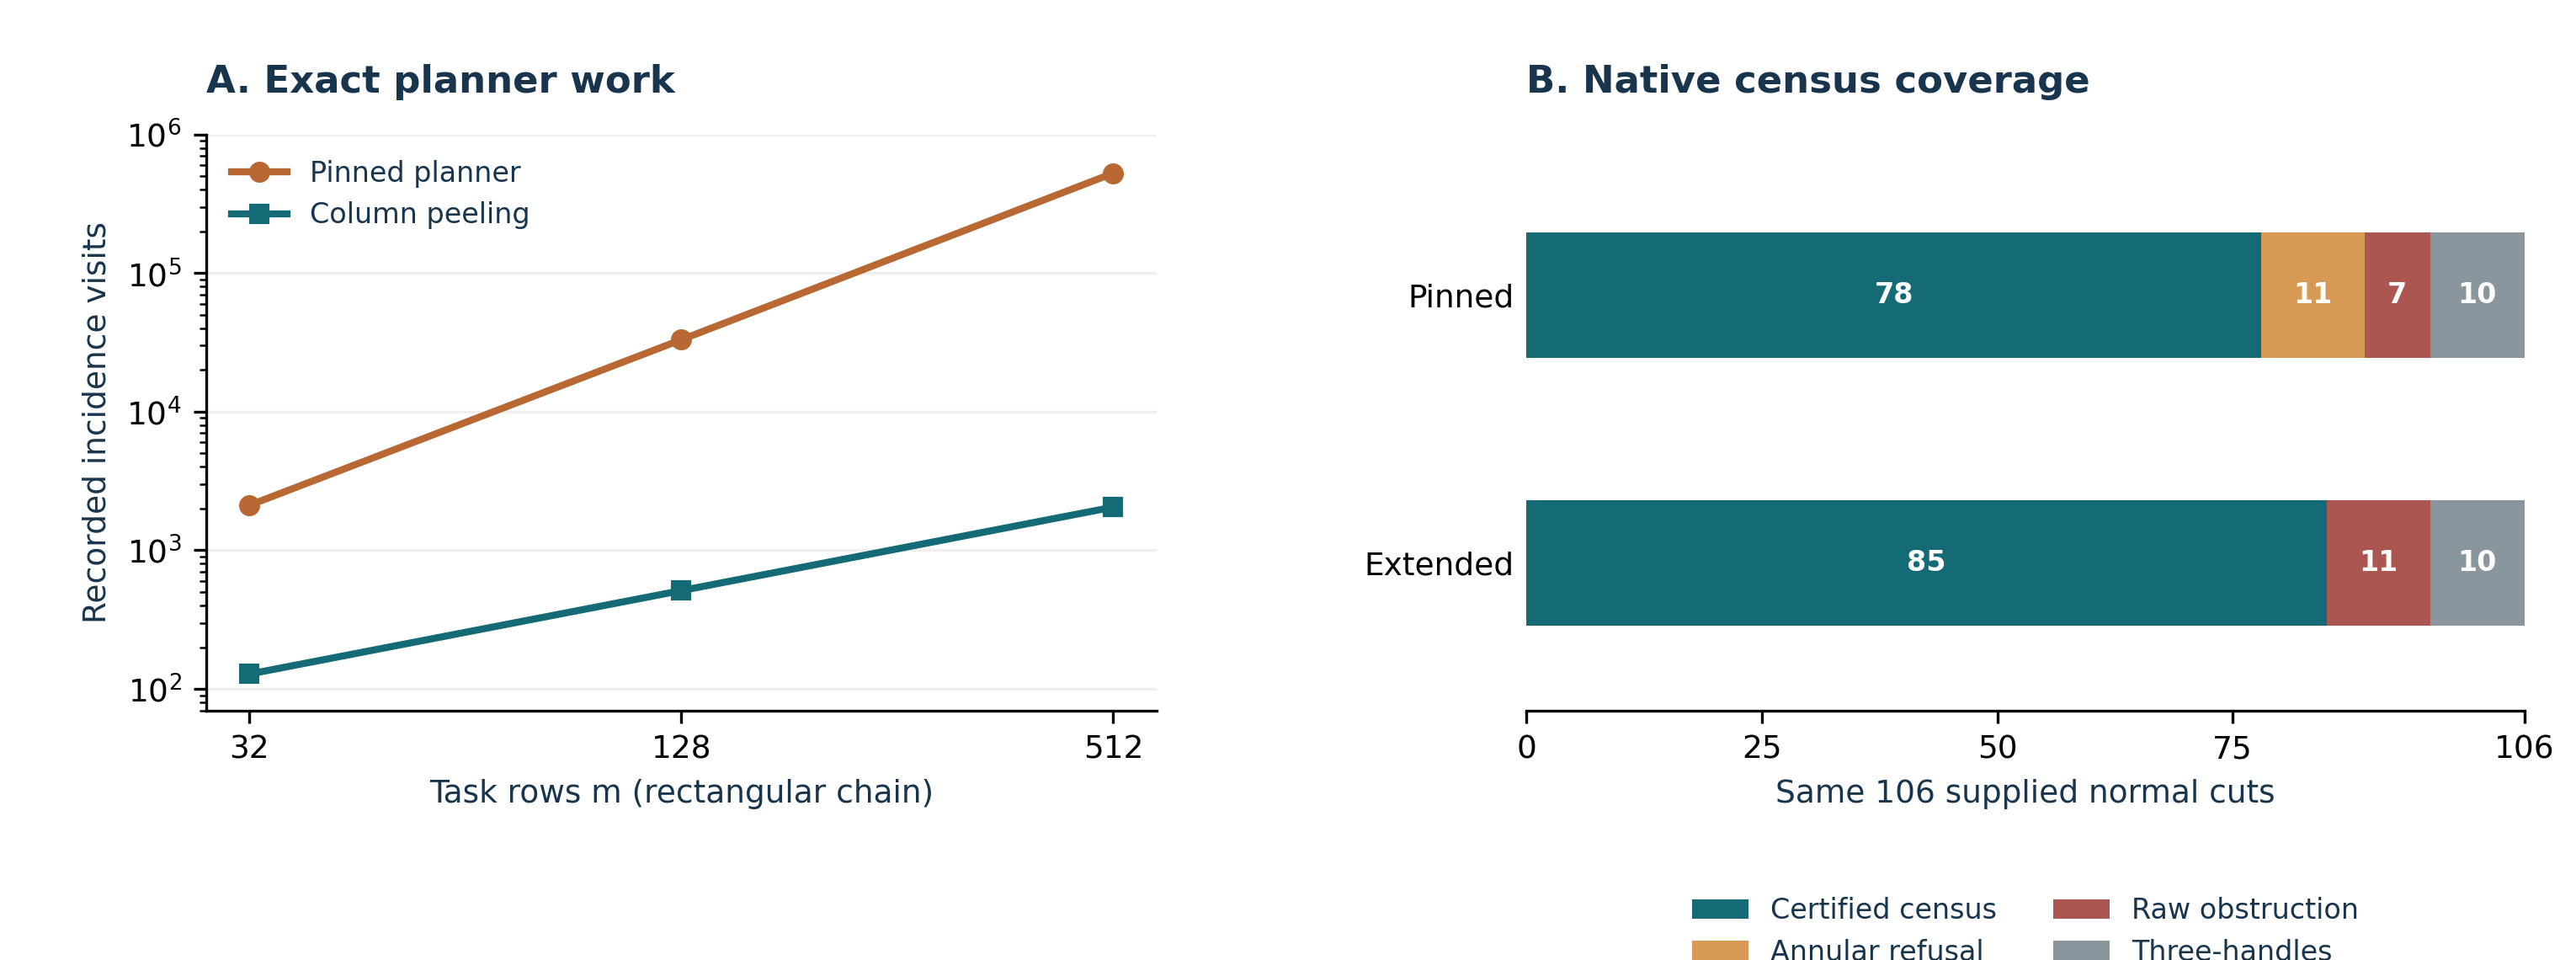
\includegraphics[width=\linewidth]{figures/work_and_coverage.png}
\caption{Left: exact recorded incidence work on rectangular chains,
including both source and deletion visits for the new method.  Right:
complete classification of the same 106 native source cases by each
consumer.  Numerical speedups on the left and topological coverage on the
right measure different improvements.}
\label{fig:work-coverage}
\end{figure}

The paired kernel timings used seven alternating-order rounds, with
separate A/A repetitions of the unchanged baseline and independent replay
timed separately.  They ran after the baseline regression process had
exited.  The following 128-row samples had comparatively stable controls.

\begin{table}[htbp]
\centering\small
\begin{tabular}{@{}lrrrr@{}}
\toprule
128-row family & Old ms & New ms & Old/new & A/A\\
\midrule
Rectangular chain & 8.424 & 0.293 & 28.73 & 1.004\\
Rectangular fan & 7.477 & 0.269 & 27.78 & 1.001\\
Cyclic stopping core & 5.075 & 0.102 & 49.73 & 1.024\\
\bottomrule
\end{tabular}
\caption{Medians for the planner kernel on Python 3.12.14.  Source-matrix
construction and JSON output are untimed.  Full raw samples and the
separate verifier times are preserved.}
\end{table}

The 512-row timing ratios are also retained, but their A/A controls range
from 1.070 to 1.194.  That variation is why exact work counts, rather than
the largest wall-time ratios, carry the asymptotic conclusion.

\subsection{Complete native calls and the optional precheck}

The whole-cut timings include source reconstruction.  In the verified
task, each repetition creates a fresh certificate and independently replays
it.  Module import, corpus-file loading, and JSON output are excluded.
All calls ran sequentially after the audits had finished; seven alternating
rounds and A/A controls were used.  The controls measure variability in
this shared execution environment, rather than claiming dedicated hardware.

\begin{table}[htbp]
\centering\small
\begin{tabularx}{\linewidth}{@{}Yrrrr@{}}
\toprule
Verified common-success task & Old ms & New ms & Old/new & A/A\\
\midrule
\texttt{pilot/fibonacci\_lst\_01/0} & 1.952 & 1.866 & 1.046 & 0.943\\
\texttt{fibonacci\_lst\_05/mixed} & 107.069 & 104.351 & 1.026 & 0.960\\
\texttt{relabel/4/0} & 432.042 & 444.604 & 0.972 & 1.003\\
\texttt{binary/1/500} & 7.438 & 7.726 & 0.963 & 1.011\\
\bottomrule
\end{tabularx}
\caption{The old and new consumers perform the same complete census task.
The final two rows are regressions in this sample.  Source discovery and
source replay dominate these small active matrices.}
\end{table}

These common-success measurements do not support a broad end-to-end speedup
claim.  The verified ratios range from 0.963 to 1.046, and several controls
show comparable variability.  The gain in positive coverage is the new
geometric construction, while the large kernel ratios apply to growing
incidence families rather than every native input.

The optional precheck gives a different, direct whole-call improvement.
On all 106 inputs it preserves the 85 successful certificates exactly.
It produces six early original-core obstruction proofs.  Five inputs
actually avoid two boundary orbit queries each, for ten avoided queries
in total.  The sixth, \texttt{pilot/finite\_trefoil/0}, has no ports, so
the original boundary stage already made zero orbit queries; only later
finite work is skipped there.

\begin{table}[htbp]
\centering\small
\begin{tabularx}{\linewidth}{@{}Yrrrr@{}}
\toprule
Verified obstruction task & Full path ms & Precheck ms & Ratio & A/A\\
\midrule
\texttt{pilot/fibonacci\_lst\_04/0} & 49.713 & 21.953 & 2.265 & 0.910\\
\texttt{pilot/fibonacci\_lst\_10/0} & 97.903 & 51.890 & 1.887 & 1.002\\
\texttt{pilot/lst\_4\_9/0} & 32.936 & 16.124 & 2.043 & 0.989\\
\texttt{pilot/finite\_trefoil/0} & 5.137 & 2.866 & 1.792 & 0.981\\
\bottomrule
\end{tabularx}
\caption{Equivalent refusal of this raw certificate method.  The early
proof establishes an original-core stopping subset and avoids compiling
the full residual matrix; it does not claim to output that matrix's
canonical residual.  The first A/A control is noticeably less stable.}
\end{table}

The stopping-set theorem justifies the skipped work.  Thus the two-query
savings are exact and the roughly twofold verified-call reductions in
these samples have an identified cause.  They remain measurements of
supplied-cut tasks, not of a complete unknot recognizer or a distribution
of arbitrary knot diagrams.

\section{Retaining ambient surfaces through ordinary compression}
\label{sec:seam-repair}

The saturated-bundle operator concerns the topology of a supplied cut.  A
different obstruction to a fast hierarchy algorithm is repeated replacement
of later surfaces after an earlier surface is compressed.  The hierarchy
algorithm of~\cite[Sections~6 and~9]{lackenby2026} uses precisely such a
replacement step.  This section gives an additive repair bound for a
restricted, explicitly stated situation: the cut-open surfaces are the
pieces of a certified family of surfaces in one fixed ambient manifold.
The result does not construct the required families or provide a new
unknot-recognition algorithm.  Its purpose is to identify geometric data
under which the choice of every later ambient surface can be retained.

\subsection{The additional gluing obligation}

An ordinary sequential hierarchy does not automatically supply simultaneous
ambient surfaces.  After an earlier cut, a later surface can have unrelated
boundary traces on the two copies of the cutting surface.  Changing that
earlier surface can expose attachments on its opposite side which were
absent from the side on which a compression disk was found.  A list of
homology vectors does not record this information.

We use a \emph{surface atlas} to mean a concrete PL cut-and-reglue
presentation, with the surface pieces labeled and cooriented, and with the
following additional conditions.  Traces bearing the same label agree
under every specified face identification.  Every internal boundary arc is
paired exactly once; unpaired boundary lies on the true boundary of the
ambient manifold.  Coorientations agree across the identifications.
Distinct patches of a single label have disjoint interiors.  At the
identified edges and corners, the link of each label is a single embedded
circle at an interior surface point, or a single properly embedded interval
at a boundary surface point, in the corresponding ambient link.

These are conditions on actual charts and gluing maps.  In an explicit
finite refinement they are finite incidence and link tests.  No verifier
for an arbitrary binary-compressed surface atlas is implemented here.

In the following, a \emph{cut-open face} is a connected part of a labeled
surface cut along its intersections with the other surfaces, realized on
one boundary side of a cut piece.  It can have positive genus or several
boundary components; it is not required to be a polygon.  Its interior
maps injectively into the corresponding ambient surface.  A \emph{seam}
is an actual trace of one of the other cutting surfaces.  Auxiliary
subdivision edges in the atlas are not seams.  Thus essentiality below is
tested in the whole cut-open face, even when it is authenticated using
many polygon charts.

\begin{lemma}[What an authenticated atlas supplies]
\label{lem:seam-atlas}
Under the preceding conditions, the quotient of the patches with any one
label is a properly embedded cooriented PL surface.  In an orientable
ambient manifold it is oriented.  Suppose an embedded disk in one cut
piece has interior disjoint from its boundary faces, and has boundary in
the interior of a single cut-open face of one label, disjoint from
all seams and other labels.  Its image under regluing is an embedded disk
whose interior avoids the whole surface family and whose boundary meets
only that labeled surface.
\end{lemma}

\begin{proof}
At a patch interior the required local surface chart is already supplied.
Across an identified face, the paired traces give two compatible local
halves of a surface.  The edge and corner link conditions supply the local
product charts at the remaining points; in particular they exclude
branching, self-intersection, and an unpaired internal boundary.  The
boundary condition identifies the resulting surface boundary with a subset
of the true manifold boundary.  The coorientations glue, and an ambient
orientation converts a coorientation into a surface orientation.

Regluing is injective on the interior of each cut piece.  On the boundary
of the stated disk, it is injective because this boundary lies inside one
cut-open face whose interior embeds in its labeled ambient surface.
No interior point of the
disk can be identified with a boundary point: the former is off the
surface family and the latter lies on it.  The disk image is therefore
embedded.  The same conditions show that it meets no other labeled
surface and meets its own label only along its boundary.
\end{proof}

The local link tests in Lemma~\ref{lem:seam-atlas} must not be omitted.
Agreement of formal boundary chains alone would allow a branched or
immersed quotient.  Conversely, once the ambient surfaces have been
authenticated, the repair theorem below is purely geometric and does not
depend on a particular triangulation of them.

\subsection{A potential for one fixed ambient family}

Let $M$ be a compact orientable irreducible $3$-manifold, and let $P$ be a
boundary pattern.  Let
\[
                         \mathcal F=(F_1,\ldots,F_k)
\]
be connected oriented surfaces properly embedded in $M$, in general
position and transverse to $P$.  Assume that the classes
$[F_1],\ldots,[F_k]$ are linearly independent in
$H_2(M,\partial M;\mathbb Q)$.  Pairwise intersections are finite unions
of arcs and circles.  Triple intersections, if present, are included in
the atlas; they do not split a component of a pairwise intersection.

Use the pattern complexity from~\cite[Section~3]{lackenby2026}, measured
against the fixed original pattern $P$:
\begin{equation}
 c_P(F_i)=-4\chi(F_i)+|\partial F_i\cap P|,
 \qquad
 \iota(\mathcal F)=
       \sum_{1\le i<j\le k}\#\pi_0(F_i\cap F_j).
 \label{eq:seam-complexities}
\end{equation}
Here $\#\pi_0$ counts geometric connected components, with no algebraic
cancellation.  The pattern in~\eqref{eq:seam-complexities} is not the
changing pattern of an intermediate cut.

\begin{lemma}[Negative complexity and a nonzero relative class]
\label{lem:seam-negative}
Let $F$ be a connected oriented surface properly embedded in $M$ with
$[F]\ne0$ in $H_2(M,\partial M;\mathbb Q)$.  If $c_P(F)<0$, then $F$
is a violating disk for $(M,P)$.
\end{lemma}

\begin{proof}
A connected orientable surface of negative pattern complexity is either
a sphere or a disk meeting $P$ at most three times.  An embedded sphere
bounds a ball by irreducibility, so its relative homology class is zero.
This contradicts the nonzero-class assumption.  If a disk is not violating,
the definition supplies a disk in
$\partial M$ with the same boundary and with the permitted empty, arc, or
tripod intersection with $P$.  Together the two disks bound a ball, after
the usual small boundary perturbation, by irreducibility.  The original
disk is boundary-parallel and represents zero in relative homology,
again contradicting the hypothesis.  Thus the disk is violating.
\end{proof}

Accordingly, suppose throughout a nonterminal stage that every
$c_P(F_i)$ is nonnegative.  Define
\begin{equation}
                  Q(\mathcal F)
                  =\sum_{i=1}^k c_P(F_i)+\iota(\mathcal F).
                  \label{eq:seam-potential}
\end{equation}
This is a nonnegative integer.  The intersection term is essential: a
loop can be essential in a cut-open face while bounding a disk in its
uncut ambient surface.  Such a loop leads to a disk exchange, rather
than to a reduction in the surface's Euler characteristic.

\begin{theorem}[Ordinary compression repair in an ambient block]
\label{thm:seam-repair}
Assume the preceding hypotheses and an authenticated atlas for
$\mathcal F$.  Suppose a disk $D$ in one of its cut pieces satisfies the
disk hypotheses of Lemma~\ref{lem:seam-atlas}, and that its boundary
$\alpha$ is essential in that cut-open face, which has label $j$.
Then one can either obtain a violating disk for $(M,P)$ or replace
$F_j$ by a connected oriented proper surface $G$, retaining all the
other ambient surfaces, such that their $k$ relative classes remain
independent and
\[
                   Q(F_1,\ldots,G,\ldots,F_k)
                      <Q(\mathcal F).
\]
More precisely:
\begin{enumerate}
\item If $\alpha$ is essential in the ambient surface $F_j$, then
      $G$ can be chosen among the components of the compression of
      $F_j$ along $D$, and in the nonterminal case
      \[
          c_P(G)\le c_P(F_j)-4,
          \qquad \iota(\mathcal F_{\mathrm{new}})
                         \le\iota(\mathcal F).
      \]
\item If $\alpha$ bounds a disk in the ambient $F_j$, then $G$ can
      be obtained by a disk exchange.  It has the same relative class,
      Euler characteristic, and boundary as $F_j$, while
      \[
                     \iota(\mathcal F_{\mathrm{new}})
                         <\iota(\mathcal F).
      \]
\end{enumerate}
\end{theorem}

\begin{proof}
By Lemma~\ref{lem:seam-atlas}, regluing gives an embedded disk in $M$
meeting $F_j$ exactly in its boundary and avoiding every $F_i$ with
$i\ne j$.  We continue to denote this image by $D$.  A sufficiently
small surgery neighborhood of $D$ is disjoint from the other surfaces.

First suppose that $\alpha$ is essential in $F_j$.  Let $F'_j$ be the
oriented surface obtained by compression.  The surgery trace gives
\begin{equation}
                   [F'_j]=[F_j]
                   \quad\hbox{in }H_2(M,\partial M;\mathbb Q).
                   \label{eq:seam-class}
\end{equation}
Write $V$ for the span of the other $k-1$ classes.  At least one
connected component $G$ of $F'_j$ has $[G]\notin V$, since otherwise
their sum~\eqref{eq:seam-class} would belong to $V$.  Choosing such a
component preserves rank $k$.  In particular $[G]\ne0$.  If
$c_P(G)<0$, Lemma~\ref{lem:seam-negative}, with the newly independent
family, supplies the asserted violating disk.

For the remaining case we prove the quantitative drop, including the
effect of a possibly discarded component.  Compression increases total
Euler characteristic by two and leaves the boundary and its intersections
with $P$ unchanged.  Consequently
\begin{equation}
                       c_P(F'_j)=c_P(F_j)-8.
                       \label{eq:seam-eight}
\end{equation}
There are at most two components.  No component is a sphere.  Indeed, a
separating compression would produce a sphere only if $\alpha$ already
bounded a disk in $F_j$, contrary to this case.  A nonseparating
compression produces a sphere only when $F_j$ is a closed torus.  Then
\eqref{eq:seam-class} and irreducibility would force $[F_j]=0$, again
contrary to independence.

Every connected sphere-free orientable surface has Euler characteristic
at most one, so a discarded component, if present, has pattern
complexity at least $-4$.  Subtracting that complexity
from~\eqref{eq:seam-eight} yields
$c_P(G)\le c_P(F_j)-4$.  All intersections with the other surfaces
are disjoint from the surgery neighborhood.  Each lies entirely in a
component of the compressed surface, because it misses the compressed
circle.  Selecting $G$ therefore deletes entire pairwise intersection
arcs or circles and introduces none.  This proves the first case.

Now suppose that $\alpha$ bounds a disk $E\subset F_j$.  It must
contain a pairwise intersection circle: if its interior missed every
other surface, it would lift to a disk in the same cut-open face,
contradicting the essentiality hypothesis there.  Since $\alpha$ is
disjoint from the other surfaces and $E$ lies in the interior of
$F_j$, every pairwise intersection component meeting $E$ is a whole
circle contained in its interior.

The embedded sphere $E\cup D$ bounds a ball $B$ by irreducibility.
The connected surface $F_j\setminus\operatorname{int}E$ lies outside
this ball.  If it lay inside, then in the closed-surface case the whole
$F_j$ could be pushed into $B$, forcing its relative class to be zero.
In the case with boundary, its boundary on $\partial M$ rules out that
possibility, since $B$ is bounded by a sphere in the interior of $M$.
Thus the usual disk exchange across $B$ replaces $E$ by a small
parallel copy of $D$ while retaining an embedded oriented proper
surface.  The isotopy may pass through other members of the family;
their mutual disjointness during the isotopy is not a hypothesis.

The replacement disk is disjoint from all the other surfaces.  It
therefore deletes every intersection circle in $E$ and creates no new
intersection.  At least one circle is deleted.  The surface's relative
class, Euler characteristic, and boundary are unchanged.  This proves
the second case, and hence the strict decrease of
\eqref{eq:seam-potential} in either nonterminal case.
\end{proof}

\begin{corollary}[Additive bound for the specified repairs]
\label{cor:seam-budget}
Starting from one family satisfying the theorem, any sequence of its
specified nonterminal repairs has length at most
\[
             \left\lfloor\frac{C_0}{4}\right\rfloor+I_0,
 \qquad C_0=\sum_i c_P(F_i^{\mathrm{initial}}),
 \qquad I_0=\iota(\mathcal F_{\mathrm{initial}}).
\]
This is at most $Q(\mathcal F_{\mathrm{initial}})$.  If the last repair
instead terminates by producing a violating disk, the total number of
repairs is at most
$\lfloor C_0/4\rfloor+I_0+1$.
\end{corollary}

\begin{proof}
The $k$ classes remain independent.  At each nonterminal stage their
pattern complexities are nonnegative.  Each nonterminal compression
along a curve essential in its ambient surface reduces their sum by at
least four; disk exchanges preserve that sum.  There can therefore be at
most $\lfloor C_0/4\rfloor$ such compressions.  Each disk exchange
decreases the intersection count by at least one, and a compression never
increases that count.  There can consequently be at most $I_0$ disk
exchanges.  Adding these distinct operation counts proves the claimed
bound.  A terminal surgery is allowed to leave the nonnegative-complexity
regime, so it is counted separately.
\end{proof}

\begin{corollary}[Retaining individually nonzero labels]
\label{cor:seam-nonzero}
The geometric repair and additive bound remain valid if mutual
independence is replaced by the weaker assumption
\[
               [F_i]\ne0\quad\text{for every }i.
\]
In this version every retained label has a connected representative with
nonzero relative class.  No mutual independence conclusion is asserted.
The number of labels is unrestricted by the dimension of the homology
group.  As before, the initial stage is nonterminal only if all its
pattern complexities are nonnegative.
\end{corollary}

\begin{proof}
For an essential compression, the oriented sum of the classes of its
components is the nonzero class $[F_j]$.  Hence at least one component
$G$ has nonzero class.  Choose that component.  The exclusion of sphere
components in the proof of Theorem~\ref{thm:seam-repair} uses only
$[F_j]\ne0$ and irreducibility.  The resulting estimate
$c_P(G)\leq c_P(F_j)-4$ is therefore unchanged.  If $c_P(G)<0$,
Lemma~\ref{lem:seam-negative} still produces a violating disk.
Otherwise the same intersection argument proves a strict decrease of
$Q$, and all labels still have nonzero classes.

In the disk-exchange case, the only homological input was that $F_j$
cannot be pushed into a ball.  Its nonzero class supplies exactly that
input.  The exchange preserves its individual class and strictly
decreases the intersection term.  The separate compression and
disk-exchange counts in Corollary~\ref{cor:seam-budget} are therefore
unchanged: at most $\lfloor C_0/4\rfloor+I_0$ nonterminal repairs
and at most one additional terminal repair.
\end{proof}

Keeping every component of $F'_j$ as one labeled oriented surface would
preserve the individual class $[F_j]$.  The connected-component selection
used in the theorem preserves independence and the number of labels, but
need not preserve that individual class.  This distinction matters if a
later construction requires one fixed cohomology basis rather than merely
an independent family.

\subsection{What the additive estimate does not establish}

\paragraph{Ambient retention still requires updated cut data.}
The unchanged objects are the other surfaces embedded in $M$.  Their
pieces in the successive cuts, the induced boundary patterns, and their
source certificates can change.  Discarding one compressed component can
glue together several old pieces of a later surface.  The theorem therefore
permits retaining ambient surface choices; it does not justify reusing
old normal coordinates, handle structures, source digests, or suffix
certificates without verification.

\paragraph{The disks have restricted boundary behavior.}
The hypotheses cover an ordinary compression whose boundary stays in one
surface face and misses every seam.  They do not cover general
pattern-compressions involving arcs on the original boundary or several
labeled faces.  Such an extension must account for the changed pattern
intersections and for the reconnection of seam traces.  Nor does the theorem
find all the disks it permits.

\paragraph{No simultaneous normalization bound is supplied.}
The repaired surfaces need not be normal in the previous handle structure.
Normalizing one of them can change its intersections with the others.  To
use Corollary~\ref{cor:seam-budget} inside a normal-surface algorithm, one
would need to control that change or charge it to another bounded
quantity.  Likewise, irreducibility proves that the disk-exchange ball
exists; this proof supplies no bound for a compressed description of the
resulting isotopy.

\paragraph{The potential is geometric, not automatically polynomial in
the input bit length.}
For example, take the two vertical annuli in $T^2\times I$ above curves
of slopes $(1,0)$ and $(1,N)$ in minimal position.  Their pattern
complexities for $P=\varnothing$ are zero, but their pairwise intersection
has $N$ arcs.  A slope or twist description can store $N$ in binary.
Thus even an additive bound in $Q$ can be exponential in a compressed
description length.  The example illustrates the size of the bound; it
does not assert that these annuli actually require $N$ repairs.

\paragraph{Homological independence has limited force.}
The preserved assertions are embeddedness, orientation, properness,
connectedness of each selected representative, and independence in the
fixed ambient relative homology group.  The theorem asserts neither
incompressibility nor pattern-incompressibility.  It also does not prove
nonseparation of every later cut-open surface after several previous cuts,
or the $q$-complexity descent required by the hierarchy algorithm.

For the independent version there is also a strict rank restriction:
$k\leq\dim H_2(M,\partial M;\mathbb Q)=b_1(M)$ by
Poincar\'e--Lefschetz duality.  For a knot exterior, abelianizing a
Wirtinger presentation identifies all arc generators with one meridian
generator, so $b_1(M)=1$.  The independent version consequently cannot
retain a whole multisurface hierarchy in the original knot exterior.
Its multiple-label use requires an appropriate later ambient block of
larger first Betti number and a suitable atlas there.
Corollary~\ref{cor:seam-nonzero} avoids this rank restriction by retaining
only individual nonzero classes, and so permits several ambient labels
even in a knot exterior.  Neither version proves that the resulting
pieces form a valid sequential hierarchy.  In particular, the corollary
does not replace the missing later-cut nonseparation argument.

The resulting research problem is concrete.  Construct ambient atlases
whose geometric intersection complexity is controlled, authenticate their
seams without expanding binary multiplicities, and retain that control
through simultaneous normalization and pattern-compression.  The local
cutting and bundle results, including the incoming relative-handle
work~\cite{incoming-hierarchy-kernels}, address different parts of this
construction.  The additive repair theorem does not close those remaining
obligations or imply a global quasi-polynomial recognition bound.

\section{A proposed research program}
\label{sec:research-program}

The next work should target proof obligations exposed by the construction,
not merely increase the number of heuristic moves attempted.  We propose
the following program, arranged from the nearest implementable extension
to the missing global complexity theorem.  Each question includes a
concrete outcome by which progress can be judged.

\subsection{Immediate geometric and implementation questions}

\paragraph{1. Can a canonical raw obstruction guide geometric normalization?}
The residual stopping set identifies precisely which original and saturated
rows cannot disappear in the fixed model.  For the eight retained native
positive cuts with raw obstructions, locate a source-authenticated move
that changes one of these rows' actual cocore intersections.  Candidates
include boundary bigon removal, a different meridian disc system, and a
small certified change of the core handle structure.  The outcome should
be a before/after geometric certificate and a strictly smaller stated
measure, rather than a freely reduced relator that happens to contain
a singleton.  This is a finite, already supplied test set on which a
successful next theorem would have visible consequences.

\paragraph{2. How can geometric unit intersections be discovered efficiently?}
An algebraic exponent of one is insufficient.  One needs an embedded
attaching curve, an actual meridian disc, and a controlled isotopy or disc
slide proving one geometric intersection.  Lackenby's curve algorithms
compute geometric intersection and isotopy information in polynomial
time in surface triangulation size and logarithmic curve weights
\cite{lackenby-curves}.  The research task is to connect their exact input
and output structures to the source boundary charts here.  A separate
minimum-intersection calculation for each pair of curves would not by
itself certify one simultaneous complete meridian system.

\paragraph{3. Which three-handle cores admit compressed cancellation?}
Seven of the ten retained three-handle cases are actual unions of
handlebodies according to the explicit oracle.  Develop a source verifier
for a safe two/three-handle cancellation or a controlled retriangulation,
including how every bundle port is transported.  Start with these seven
cases and retain the three negative controls.  A sphere boundary or an
Euler calculation must not authorize deletion of a closed summand.
An eventual theorem should bound the number of new source records, not
only the change in Euler characteristic.

\paragraph{4. Can private cocores be addressed without being enumerated?}
The present theorem supplies their count and initial incidence type, but
not a name for every cocore in a genus-$2^B$ bundle.  A useful extension
would provide a parameterized family of cocores with a bounded number of
chart types, a binary address within each family, and independently
checkable intersection queries.  Its output contract should allow finite
queries rather than require a literal list of all handles.  The initial
target can be patterns using only polynomially many source ports; the
general case must allow the possibility of larger representation costs.

\paragraph{5. What boundary-pattern information survives the compression?}
An unmarked genus histogram omits cyclic order, endpoints, coorientation,
and the placement of graph vertices.  Design a richer certificate that
retains this data through the collar construction, connector contractions,
and geometric cancellations.  Matching the genus and a matrix of unsigned
intersections is not an adequate test.  A strong validation target is an
independent reconstruction of the induced pattern on small explicit cut
boundaries, followed by exact agreement of essential-pattern tests.

\paragraph{6. Can the finite compiler be made linear in its explicit input?}
The new peeling pass is linear in incidence work, but the delivered
relative component assembly and independent forest reconstruction are
deliberately straightforward polynomial routines.  Index each row, port,
and base once by its component, and replace repeated scans by one grouped
pass.  Preserve the independent checker architecture rather than importing
the producer's union--find routine.  Measure the complete verified task:
the current common-success timings show that optimizing a small finite
subroutine may have little effect when orbit discovery dominates.

\subsection{Compressed geometric transitions}

\paragraph{7. Can the incoming cut grammars compile actual hierarchy moves?}
The incoming tile and first-return results already evaluate important
compressed local queries\cite{incoming-disconnected,incoming-sparse,incoming-moments}.
The next theorem should start with authenticated source charts and end
with the exact charts of the modified manifold, including the new boundary
pattern.  Each grammar edge needs a geometric carrier; each gluing needs
orientation and endpoint checks.  A polynomial evaluation bound for an
already supplied grammar is only one part of this transition theorem.

\paragraph{8. When does a sequential hierarchy admit an ambient block atlas?}
Theorem~\ref{thm:seam-repair} assumes an atlas; it does not construct one
from arbitrary later surfaces.  Characterize the obstruction to matching
opposite boundary traces when those surfaces are reglued into an earlier
manifold.  An algorithm should either produce a properly embedded ambient
family with verified local links, or exhibit the unmatched seam or
self-intersection that prevents such a family.  This makes the extra
hypothesis testable rather than treating it as an informal picture.

\paragraph{9. Can many seam exchanges be batched with a real decrease bound?}
The sharpened repair estimate is
$\lfloor C_0/4\rfloor+I_0$, and $I_0$ can be exponentially large in a
binary slope description.  Seek a theorem that removes a whole certified
parallel family of intersection circles in one compressed operation, with
an amortized bound on the number of family changes.  Merely storing $I_0$
in binary or taking its logarithm does not change the number of unit
repairs.  The output should include the new surface carriers and a proof
that no remaining seam is reconnected incorrectly.

\paragraph{10. Can normalization respect the block potential?}
Ordinary repair leaves standard embedded surfaces that need not be normal
in the current handle structure.  Normalizing one while ignoring the
others can increase intersection complexity.  Prove either simultaneous
normalization with controlled $\sum c_P+\iota$, or a second bounded
quantity paying for every increase.  The individually nonzero variant
of the repair theorem allows many labels even in a knot exterior, but
does not guarantee that every later cut-open surface is nonseparating.
That sequential admissibility condition must be checked separately.

\paragraph{11. Can the component-selection step be performed from orbit data?}
The repair proof selects a compression component with nonzero relative
class, or one outside the span of the other classes.  To implement that
selection without expanding sheets, enrich the component oracle with
authenticated relative homology weights and orientation data.  Verify
that the weights really add under regluing and that the selected component
has the claimed boundary carrier.  A vector of abstract homology labels
without such carriers would not establish the embedded atlas hypotheses.

\subsection{The genuinely global questions}

\paragraph{12. Can useful surfaces be found within the intended candidate budget?}
A short certificate and a fast cut consumer do not bound discovery.
Establish a coverage theorem for a specific family of normal or compressed
surfaces: every eligible hierarchy state must contain a useful candidate
within a stated, efficiently searchable family.  The theorem must control
both the number of alternatives and their encoded sizes.  This is the
place to connect the earlier sparse-support and tile kernels to the
selection problem, rather than treating those kernels as an enumeration
bound.

\paragraph{13. Is there a logarithmic-depth structural decomposition?}
To obtain the February exponent by
Theorem~\ref{thm:conditional-composition}, one sufficient target is
$L=O(\log n)$ with polynomial candidate and state bounds.  The March
exponent permits $L=O((\log n)^2)$ under the same hypotheses.  Seek a
structural operation that decreases a suitable charged complexity by a
fixed proportion, or an amortized substitute.  A proof that a positive
integer decreases by one gives termination and a linear numerical bound,
which is not a logarithmic-depth theorem.

\paragraph{14. Can backward corrections be charged without resetting a full suffix?}
The ambient-block theorem demonstrates one sufficient local condition
for retaining other surface choices.  The next global result would have
to decompose every relevant correction into such blocks, control the
number and cost of block changes, and cover pattern-compressions and
vertical-boundary moves.  The goal is an honest replacement for the
reset factor $(g+1)^L$, with a potential maintained across all those
operations.  Counterexamples in which a later surface cannot be reglued
should be collected alongside successful block repairs.

\paragraph{15. Can all encoded-size bounds be composed from the diagram?}
Maintain a ledger for triangulation records, pattern records, normal
coordinate bits, private-family descriptions, and certificate trace size
after every operation.  Prove a bound in the original crossing count,
including transitions that simplify topology but enlarge its encoding.
Only after discovery, transport, and reset costs fit one such ledger can
the local results legitimately enter a global quasi-polynomial theorem.
The final test is a proof of the hypotheses of
Theorem~\ref{thm:conditional-composition}, or a different complete cost
argument, rather than an extrapolation of the benchmark curves.

\subsection{Proposed order of work}

The nearest next contribution is geometric normalization of the eight
retained raw-positive failures, paired with a source-preserving
two/three-handle rule for the seven retained three-handle positives.
These tasks have concrete source cases, exact oracles at small scale,
and a clear success criterion.  Boundary-pattern transport and private
cocore addressing should proceed alongside them, because an unmarked
terminal result alone cannot drive the intended hierarchy.  Ambient
block construction and batched repairs then address the reset bottleneck.
Candidate coverage and global size/depth control remain the final
structural obligations.

\appendix
\section{Reproduction and integration package}
\label{sec:reproduction}

The accompanying archive includes this PDF and all \LaTeX{} sources, the
new producer and verifier modules, tests, raw source cases and certificates,
the unchanged pinned runtime required by the examples, baseline comparison
code, experiment scripts, and an additive integration patch.  No remote
repository branch has been changed by this continuation.

\subsection{Minimal commands}

From the extracted package root, run the standard-library extension tests:
\begin{verbatim}
PYTHONPATH=code:runtime python3 -B -m unittest discover -s tests -v
\end{verbatim}
This includes all 106 precheck on/off comparisons and source replays.
The recorded run used Python 3.12.14.  The optional explicit-cut audit
additionally needs Regina, recorded as version 7.4:
\begin{verbatim}
PYTHONPATH=code:runtime python3 -B experiments/native_audit.py
\end{verbatim}
It repeats the old/new comparison and literal-cut oracle, retaining the
normal-disc expansion cap.  To replay the saved certificates without
rerunning discovery or the oracle, use:
\begin{verbatim}
PYTHONPATH=code:runtime python3 -B experiments/replay_saved.py
\end{verbatim}

Run the two benchmark scripts sequentially, with other experiment and test
processes stopped:
\begin{verbatim}
python3 -B experiments/benchmark_column_peeling.py
PYTHONPATH=code:runtime python3 -B experiments/benchmark_native.py
\end{verbatim}
The comparison scripts emit raw repetition arrays and A/A controls.
Their results are local measurements and should be regenerated on the
integration machine rather than treated as machine-independent constants.

To regenerate the static figure and build the article, use:
\begin{verbatim}
python3 -B experiments/generate_figures.py
python3 -B build_article.py
\end{verbatim}
Figure generation uses Matplotlib.  The supplied PNG and SVG are already
present, so rebuilding the PDF itself requires only a normal \LaTeX{}
installation with the packages named in the main source.  The build script
runs \texttt{pdflatex} three times and preserves its log for inspection.

\subsection{Important files}

{\small
\begin{longtable}{@{}>{\raggedright\arraybackslash}p{0.46\linewidth}>{\raggedright\arraybackslash}p{0.49\linewidth}@{}}
\toprule
Path & Purpose\\
\midrule
\endhead
\path{code/column_peeling.py} and
\path{code/column_peeling_verify.py} & Sparse matrix producer and
independent timestamp/stopping-set verifier\\
\addlinespace
\path{code/relative_bundles.py} and
\path{code/relative_bundles_verify.py} & Finite geometric compiler and
independent reconstruction\\
\addlinespace
\path{code/normal_cut_saturation.py} and
\path{code/normal_cut_saturation_verify.py} & Complete source-bound
wrapper and replay, including optional early core refusal\\
\addlinespace
\path{data/native_audit.json} & All 106 baseline/new results and actual
Regina comparisons; no omitted refusals\\
\addlinespace
\path{data/core_precheck_audit.json} & Enabled/disabled comparisons,
identical success proofs, and exact query savings\\
\addlinespace
\path{data/native_benchmark.json} & Complete-call timing repetitions
and A/A controls\\
\addlinespace
\path{results/column_peeling_validation.json} and
\path{results/column_peeling_benchmark.json} & Algebraic validation
counts, exact work counters, and raw kernel timings\\
\addlinespace
\path{data/certificates/} & Seven new successes, legacy and binary
controls, a full raw obstruction, and an early core obstruction\\
\addlinespace
\path{data/extension_tests.log} and
\path{data/native_regression_pinned.log} & Final 37-method extension
run and 1,663-test pinned baseline run\\
\addlinespace
\path{integration/additive_extension.patch} & Adds namespaced modules
to the pinned repository without changing its default consumers\\
\addlinespace
\path{INTEGRATION.md} and \path{CLAIMS.md} & Proposed integration
sequence, proof obligations, and boundaries of the claims\\
\bottomrule
\end{longtable}
}

The \path{runtime/fastunknot/} files and
\path{baseline/core_handlebody_7046006.py} are unchanged excerpts of
the inspected source.  Their original licensing accompanies the package.
The main implementation can be reviewed separately from those reference
files.  The observer-family lemma and ambient-block repair theorem are
mathematical contributions only; no code in the package claims to solve
their missing geometric input or transport problems.

\subsection{A safe integration sequence}

Apply the additive patch to a checkout containing the expected source
interfaces, then import the new modules through the \texttt{fastunknot}
namespace.  Verify saved source certificates and run the added focused
tests before putting the operator behind an explicit experimental option.
Preserve the old full-row consumer while comparing census agreement and
full-call costs.  A later change to the default recognition schedule
should state which selected surfaces reach this operator and how its
unmarked census participates in the existing topological proof.

The present contribution is complete as an opt-in research operator and
reproducible article.  Its interface intentionally reports inconclusive
cases that remain outside its hypotheses or fail its fixed geometric
criterion.  Those retained cases, not a claim of general quasi-polynomial
recognition, are the basis for the next research stage.

\begin{thebibliography}{99}
\raggedright

\bibitem{ProveItPinned}
V. Reshetnikov and contributors,
\emph{ProveIt: Topology/UnknotRecognition and docs/incoming},
inspected commit \texttt{704600626606a9097cfd89d4e3d2bbc63c8dd1cb},
12 October 2026.
\href{https://github.com/VladimirReshetnikov/ProveIt/tree/704600626606a9097cfd89d4e3d2bbc63c8dd1cb/Topology/UnknotRecognition}{Pinned algorithm directory};
\href{https://github.com/VladimirReshetnikov/ProveIt/tree/704600626606a9097cfd89d4e3d2bbc63c8dd1cb/docs/incoming}{pinned incoming directory}.

\bibitem{raw-epoch-56}
ProveIt research continuation,
\emph{Saturating Raw Tietze Eliminations and Indexing Certified Interval
Orbits}, retained report 56, 9 October 2026.
In particular \path{reports/56/article/raw_epoch.tex}.
\href{https://github.com/VladimirReshetnikov/ProveIt/blob/704600626606a9097cfd89d4e3d2bbc63c8dd1cb/Topology/UnknotRecognition/reports/56/article/raw_epoch.tex}{Pinned theorem source}.

\bibitem{marked-parallelity-85}
ProveIt research continuation,
\emph{Marked Parallelity Interfaces}, retained report 85 and the maintained
synthesis chapters on source parallelity, core handlebodies, ordered
boundary words, and primitive bundle annuli, 12 October 2026.
\href{https://github.com/VladimirReshetnikov/ProveIt/tree/704600626606a9097cfd89d4e3d2bbc63c8dd1cb/Topology/UnknotRecognition/reports/85}{Pinned report directory}.
The actual comparison implementation is the maintained \texttt{fast/}
source at the inspected commit, not an earlier report snapshot.

\bibitem{incoming-hierarchy-kernels}
ProveIt research continuation,
\emph{Three Reductions for Certified Unknot Hierarchies},
12 October 2026.  Incoming archive
\path{ProveIt_Unknot_Hierarchy_Kernels_2026-10-12.zip},
especially \path{article/sections/unsaturated.tex}.
\href{https://github.com/VladimirReshetnikov/ProveIt/blob/704600626606a9097cfd89d4e3d2bbc63c8dd1cb/docs/incoming/ProveIt_Unknot_Hierarchy_Kernels_2026-10-12.zip}{Pinned archive}.

\bibitem{incoming-disconnected}
ProveIt research continuation,
\emph{Polynomial Marked-Cut Kernels for Arbitrary Disconnected Tile Powers},
12 October 2026.  Incoming archive
\path{ProveIt_Disconnected_Tile_Kernels_2026-10-12.zip}.
\href{https://github.com/VladimirReshetnikov/ProveIt/blob/704600626606a9097cfd89d4e3d2bbc63c8dd1cb/docs/incoming/ProveIt_Disconnected_Tile_Kernels_2026-10-12.zip}{Pinned archive}.

\bibitem{incoming-sparse}
ProveIt research continuation,
\emph{Sparse Small-Cut Responses for Compressed Unknot Hierarchies},
12 October 2026.  Incoming archive
\path{ProveIt_Unknot_Sparse_Cut_Grammars_2026-10-12.zip}.
\href{https://github.com/VladimirReshetnikov/ProveIt/blob/704600626606a9097cfd89d4e3d2bbc63c8dd1cb/docs/incoming/ProveIt_Unknot_Sparse_Cut_Grammars_2026-10-12.zip}{Pinned archive}.

\bibitem{incoming-moments}
ProveIt research continuation,
\emph{A One-Scalar-Census Boundary Compiler for Compressed Unknot
Hierarchies}, 12 October 2026.  Incoming archive
\path{ProveIt_Moment_Coded_First_Returns_2026-10-12.zip}.
\href{https://github.com/VladimirReshetnikov/ProveIt/blob/704600626606a9097cfd89d4e3d2bbc63c8dd1cb/docs/incoming/ProveIt_Moment_Coded_First_Returns_2026-10-12.zip}{Pinned archive}.

\bibitem{lackenby2021feb}
M. Lackenby,
\emph{Unknot recognition in quasi-polynomial time},
February 2021 UC Davis lecture slides, especially PDF pp.\ 13--14.
\url{https://people.maths.ox.ac.uk/lackenby/quasipolynomial-talk.pdf}.

\bibitem{lackenby2021mar}
M. Lackenby,
\emph{Unknot recognition in quasi-polynomial time},
March 2021 Oxford lecture slides, especially PDF pp.\ 13--14.
\url{https://people.maths.ox.ac.uk/lackenby/quasipolynomial-talk-oxford.pdf}.
This is a different version from the preceding item.

\bibitem{lackenby2026}
M. Lackenby,
\emph{Incompressible surfaces, hierarchies and unknot recognition},
arXiv:2607.23350v1, 25 July 2026.
\url{https://arxiv.org/abs/2607.23350v1}.

\bibitem{lackenby-curves}
M. Lackenby,
\emph{Some Fast Algorithms for Curves in Surfaces},
Discrete \& Computational Geometry, published 21 April 2026,
\href{https://doi.org/10.1007/s00454-026-00845-7}{doi:10.1007/s00454-026-00845-7}.
Preprint \href{https://arxiv.org/abs/2401.16056v2}{arXiv:2401.16056v2},
20 March 2026.

\bibitem{AHT2006}
I. Agol, J. Hass, and W. P. Thurston,
\emph{The computational complexity of knot genus and spanning area},
Transactions of the American Mathematical Society \textbf{358} (2006),
3821--3850.
\url{https://arxiv.org/abs/math/0205057}.

\bibitem{ReginaAPI}
B. A. Burton and the Regina development team,
\emph{Regina: Software for low-dimensional topology},
calculation-engine API documentation, accessed 12 October 2026.
\href{https://regina-normal.github.io/engine-docs/classregina_1_1Triangulation_3_013_01_4.html}{Triangulation\textless3\textgreater{} and
\texttt{recogniseHandlebody()} documentation}.
The experiment used Regina 7.4; the online documentation identifies its
current engine as 7.4.1.

\end{thebibliography}

\end{document}
